\section{Introduction}
Accessibility is a revealing indicator of many urban processes. It can take multiple forms in notionally describing mobility within an urban system \citep{muraco1972intraurban,vickerman1974accessibility}; to its use as a quantifiable benchmark to evaluate urban policies \citep{paez2012measuring,masucci2013gravity,piovani2018measuring, yang2019comprehensive}. It is a measure that is intimately linked to many different urban dimensions --- its land-use, transport structures, and resident populations \citep{miller2018accessibility}. Its utility is evident from the gained advantage of accessibility measures to computationally distil complex urban processes into interpretable metrics that can be used across geographies and scales \citep{bhat2000development}. And, as such, it has been indispensable in opening critical discourse on many real issues of resource and infrastructure provision \citep{van1999accessibility}, and land-use decisions-making \citep{tsou2005accessibility,sa2006does,cheng2013measuring, brondeel2014use}; to more systemic concerns of urban equity \citep{van1999accessibility, curl2011does}, social segregation \citep{massey1988dimensions,arapoglou2009new,li2013residential}, and planning for alternative development futures \citep{cervero1997paradigm, geurs2012accessibility}.\\

In spite of this utility, perhaps more important in the use of accessibility measures are their overarching description of equity within the urban system. \citep{hansen1959accessibility,nelson1993assessing,ihlanfeldt1994spatial}. Rightly so, where stark disparities in accessibility exist, an acute spatial mismatch can implied \citep{kain1992spatial,nelson1993assessing,ihlanfeldt1994spatial,gobillon2007mechanisms} --- of which, its presence over time is suggestive of a system that may compound and enforce certain spatial inequalities. This is a ubiquitous issues in cities globally; and, it warrants detailed consideration for numerous reasons. Unequal accessibility has tangible manifestations within a city's socioeconomic structures \citep{kain1992spatial}. Thus far, a large body of literature has already been established on its disproportionate effect, not least, on low-income and ethnic groups \citep{kain1992spatial}; but, also, on the provision of affordable housing \citep{hillier2003spatial,dujardin2005neighborhood}; the reinforcement of poverty cycles \citep{gobillon2007mechanisms,aaslund2010important}; and, the differential outcomes of demographic group that persist transgenerationally \citep{cervero1995job}.\\

Their negative ramifications, particularly on more disadvantaged demographic groups, press a strong need to further investigation. However, owing to its multifaceted nature, how these spatial inequalities can be best examined must be first discussed. Prior research have already shown that variations in accessibility within urban systems can often be reflected spatially within population structures. Examples of such structures are differential income groups, with accessibility often found to be negatively linked with lower-income groups \citep{weber2002bringing,ohnishi2011evolution,de2013explaining}. The degree to which variations in accessibility may assort itself inline with these groups is an important inquiry, which raises the question as to whether these reflections may be present in other closely linked urban dimensions. House prices come to the forefront here given its well-established links to issues of income segregation and poverty alleviation \citep{maattanen2014income}.\\ 

Perhaps understanding interplays between these key urban variables may still be a worthwhile endeavour. It can be argued to offer more clarity on whether issues of accessibility, income segregation, and house prices are common in cities globally; and, with this, it may also enable more targeted measures and interventions to be formulated and implemented, in addition to challenging current policy controls that are ineffectual. This objective forms the basis of this paper, in that it seeks to first extend the necessary discussion of the underlying mechanisms that maintain socioeconomic inequality within cities. In particular, it focuses on the spatial variation of accessibility to employment within the Greater Sydney (GS) Metropolitan area to contribute a more quantifiable spatial proof to current empirical studies. The study then investigates any existing spatial variables against income and house price data, which is assumed to be exogenous to accessibility.\\

To develop the main theoretical framework of this analysis and fulfil the above objectives, this paper is structured as follows. A review of the theoretical underpinnings of accessibility, income segregation, and house prices briefly mentioned above; as well as the adopted methodological approaches to analyses these dimensions will be provided in Section \ref{sec:operationalising}. It first provides a a short assessment on how the concept of accessibility can be operationalised and defined for analysis. It discusses the numerous established methodologies and indices that have posited in previous research. It conducts this review with respect to the implications of accessibility on employment opportunities, income segregation, and the property market (ref. Section \ref{sec:a_is_hp}). Section \ref{sec:australia} deliberates on the applicability of these theories to Australia, and, in particular, the GS area. It draws upon the insights gained from the existing literature to provide a synoptic assessment of the current limitations within the scope of this study to address. Section \ref{sec:data} details the data used in the present study. And, the analytical techniques used to explore and evaluate these datasets will be expanded on in Section \ref{sec:method}. Lastly, this paper concludes with a discussion of the main findings and their limitations in Section \ref{sec:results}. This comes in addition to its discussion on the broader role accessibility plays in planning for GS and the wider Australia region.\\

\subsection{Operationalising Accessibility}
\label{sec:operationalising}

As mentioned, accessibility is a highly complex dimension of the built-environment. In physical terms, it may refer to the ease-of-reach between locations as determined by their land-uses, the underlying transport network structures, and the intervening separation between these locations \citep{mackiewicz1996towards, handy1997measuring}. More theoretically, it may also be discussed as the magnitude of potential population movement within the urban system proportional to the level of attraction at a destination; and, this is also inverse to increasing separation  \citep{hansen1959accessibility,wilson1971family,van1999accessibility, geurs2012accessibility,miller2018accessibility}. Likewise, there are a number of different models that can be used to capture accessibility with respect to these different facets. For brevity, three relatively popular models will be reviewed and compared for their suitability in this paper.\\

At their most basic level, accessibility models concern the separation between locations. Separation, here, typically refers to physical separation; and, they are broadly termed as such, spatial-separation models \citep{bhat2000development}. The weighting placed on separation can be intuitively interpreted as a reductive mobility cost, where accessibility is negatively correlated with increasing separation \citep{miller2018accessibility}.  There is an emphasis on equity as the reduction in the cost of movement, which advocates for the spatial redistribution of essential urban and economic facilities to create functional areas that are equally proximate \citep{ingram1971concept, bhat2000development}. \\

It is a simple measure, but should not be disparaged. In recent years, such basic interpretations of accessibility has gained substantial traction in many planning and development applications. They form the tenets for the creation of the 'city of proximity', whereby the location of urban necessities and crucial economic functions are primarily constrained and evaluated within narrow time-- or distance-- thresholds \citep{bhat2000development, miller2018accessibility}. \\

Notable implementations of this can be seen globally: for example, with Portland's '20-minute neighbourhoods' and Paris' '\textit{la ville du quatre d'heure}' masterplan ambitions \citep{weber2002bringing,mcneil2011bikeability,handy2020accessibility}. In these applications, the basic spatial-separation measure is extended to account account the 'cumulative-opportunities' within a predetermined constraint \citep{bhat2000development}. Equitable accessibility is viewed as the availability of services from any one location with respect to these constraints. As indicated above, constraints may be topological or temporal. For accessibility to be maximised in this instance, an equal and homogeneous redistribution of urban functions should be pursued. This measure can be generally expressed by Equation \ref{eqn:cum_opp},

\begin{equation}
A_{i}= \begin{cases}
\sum_{j}W_{j}, & \text{if } d_{ij} \leq T \\ 0, & \text{if } d_{ij} > T 
\end{cases}
\label{eqn:cum_opp}
\end{equation}

\ldots where accessibility, $A_{i}$, is measured as the sum of destination or its corresponding attributes, $W_{j}$, at constraint, $T$. Where the intervening distance, $d_{ij}$, exceeds this parameter, a value of 0 is assigned.\\

Considering its use above, such measures allude to importance of the transport network to facilitate the availability of locations within these constraints. As such, modal dependencies are often created on its use as a metric \citep{mcneil2011bikeability,o2012spatial}. For example, measures that define accessibility with a threshold for walk-times cannot be compared with cities where there are automobile hegemonies (e.g., cities that have experienced significant decentralisation or sprawl in preceding years). Consequently, their applicability to differing city structures should be highlighted and discussed in light of these modal-dependent variations \citep{o2012spatial,miller2018accessibility}. Moreover, location planning based on the objective of equal spatiotemporal separation, as described above, can be argued as oversimplified \citep{nelson1993assessing,van1999accessibility}. It makes assumptions that the diversity, quality and capacity of different urban amenities and functions are homogeneous throughout space; although, in reality, variations between locations are unavoidable. These assumptions further confront theories of agglomeration, in that complementary urban functions have economic and social benefits by being proximate to each other. Indeed, the literature that espouses the spatial benefits of clustering complementary functions is manifold; and, this is further often understood as self-organising \citep{duranton2004micro, batty2012urban}. Assessing urban systems on the basis of such homogeneous spread of urban amenities can be therefore viewed as problematic and inapplicable.\\

The stated urban asymmetries are determined by development controls, property market forces, land prices, and the subsequent constraints on land-use and land-availability \citep{ingram1971concept, black1977accessibility}. It can be argued that these variables need to be intimated within analyses to avoid a reduced view of accessibility within city systems. This is an idea that is of particular interest to this paper's theoretical development of accessibility. It leans this paper leans towards the seminal work by \citeauthor{hansen1959accessibility} (\citeyear[p.4]{hansen1959accessibility}) where accessibility can be defined as the \textit{'potential of opportunities for interaction'} within the built-environment. In his classical model (ref. Equation \ref{eqn:hansen_generalised}),

\begin{equation}
\label{eqn:hansen_generalised}
    A_{i} = f(V_{i}, W_{j}, f(d_{ij}))
\end{equation}

\ldots, the accessibility ($A$) at location $i$ is a function of the attributes at the origin ($V_{i}$) and destination ($W_{j}$) points. The measure of separation within this relationship is represented by a distance-decay function, $f(d_{ij})$. It may encapsulate a wide range of terms to determine the separation between locations (i.e., time travelled, network or Euclidean distance, etc.). The function, itself, controls the estimation of the model flows, with the propensity for movement dropping off in a non-linear way. It may be represented in several ways; however, it is most commonly utilised with respect to a power-law ($f(d_{ij}) = d^{-\beta}_{ij}$) or negative-exponential ($f(d_{ij}) = e^{-\beta \cdot d_{ij}}$). $\beta$ is noted within the distance-decay function; and, it represents the sensitivity of the model to the effects of separation as mentioned above. It is calibrated against the observed and estimated flows within the model (ref. Section \ref{sec:method}).\\

Nonetheless, the underlying logic of this measure is that accessibility is strongly determined by the interacting attributes of origin and destinations points resulting in differential flows between locations. Considering this, these interacting flows can be adapted into the form of a gravity model (ref. Equation \ref{gravity}), 

\begin{equation}
\label{gravity}
T_{ij} = k\frac{V_{i}^{\mu} W_{j}^{\alpha}}{f(d_{ij})}
\end{equation}

\ldots where, the interaction ($T_{ij}$) between zones $i$ and $j$ is determined by their respective 'mass' terms, $V_{i}$ and $W_{j}$. $k$ in the above equation refers the constant of proportionality as the interaction computed within the model is equal to the sum of their observed flows. $\alpha$ and $\mu$ are coefficients to be estimated. This estimation procedure is detailed in Section \ref{sec:method}. The 'mass' terms refer to known origin and destination specific attributes; and, these may include variables such as total origin population or a factor for destination attractiveness (e.g., facility catchment \citep{luo2014integrating}, total floorspace \citep{piovani2018measuring}, employment capacity \citep{kantorovich1992equilibrium, hernandez2006information}, or quality of facility \citep{geurs2015recent}).\\

In later iterations of the gravity model, important contributions by \cite{wilson1971family} included the introduction of model constraints. This came in recognition that the degree of interaction may not be commensurate to a system's observed flows, whereby it was argued that the sum of interactions should equal the observed flows between locations. This can be denoted by Equation \ref{sumflows}, 

\begin{equation}
\label{sumflows}
    T = \sum_{i}\sum_{j}T_{ij}
\end{equation}

\ldots where, $T$ represents the total sum between all locations of ${i}$ and ${j}$. Following this logic constraints on the model can be intuitively appended in two ways: first, if either one of the origin and destination totals are known (i.e., singly-constrained), as seen in Equation \ref{eqn:procon} and Equation \ref{eqn:attcon}, 

\begin{equation}
\begin{matrix}
\text{With a production constraint:} & \sum T_{ij} = B_{i} \cdot O_{i} W_{j} f(d_{ij})
\end{matrix}
\label{eqn:procon}    
\end{equation}

\begin{equation}
\begin{matrix}
\text{With an attraction constraint:} & \sum T_{ij} = C_{j} \cdot V_{i} D_{j} f(d_{ij})
\label{eqn:attcon}    
\end{matrix}
\end{equation}

\ldots or, if the total flows between both origin-destination points are known (i.e., doubly-constrained), which can be illustrated by Equation \ref{eqn:pro-attrac},

\begin{equation}
\begin{matrix}
\text{With a production-attraction constraint:} & \sum T_{ij} = B_{i} \cdot C_{j} \cdot V_{i} W_{j} f(d_{ij})
\end{matrix}
    \label{eqn:pro-attrac}
\end{equation}

In the above equations, the co-variates $O_i$ and $D_j$ are introduced, wherein they are the representative mass terms at either the origin or destination locations, respectively. However, more importantly in these equations are the balancing factors for origin points, $B_{i}$, and destination points, $C_{j}$. These are introduced as fixed effects to preserve either the destination or origin attributes in the subsequent model estimates.  The estimated model flows are thus calibrated to converge on their respective constraints. In the doubly-constrained model, both are estimated reiteratively following Equation \ref{eqn:balancing_factors}. These equations also hold true for their respective singly-constrained model.

\begin{equation}
\begin{matrix}
B_{i} = \frac{1}{\sum_{j} W_{j} f(d_{ij})} &,& C_{j} = \frac{1}{\sum_{i} V_{i} f(d_{ij})}
\end{matrix}
\label{eqn:balancing_factors}
\end{equation}

It can be argued that the use of the above gravity potential model allows a more nuanced view of accessibility. It displays more sensitivity to urban externalities due to its use of both the distance decay, as well as attraction, $\alpha$, and emissivity, $\mu$, parameters (ref. Equation \ref{gravity}; \cite{wilson1971family,liu2004accessibility}). This allows the model to be interpreted intuitively as also a behavioural indicator, with the willingness to travel influenced by the cost-- and attractiveness-- of locations within urban systems based on the respective mass terms \citep{wilson1971family, miller2018accessibility}. Resultingly, it offers a more holistic view of the inherent dissimilar spatial distributions and biases present within all urban systems. Moreover, its predication on prevailing land-use patterns and existing transport system across multiple spatial and modal levels may perhaps have value in informing decision-making across multiple offices \citep{ewing2002measuring,karou2012accessibility,haynes2020gravity}. This utility will also be explored more within the present study.\\

% Need more detail perhaps

\subsection{Accessibility, Income Segregation and House Prices}
\label{sec:a_is_hp}

The above sections have now  briefly touched on the many variable effects of accessibility. Thematically, the discussion presented issues of persistent segregation, land-use constraints, and alluded to hurdles for upward mobility amongst disadvantaged demographic groups. These are but just a few features noted most prominently in the existing literature \citep{geurs2004accessibility,ferrer2018sustainable}; and, how they each contribute to urban equity in line with accessibility should be explored further. Indeed, differential accessibility and its varied impacts represent crucial pieces of information for numerous reasons. It fundamentally upholds the established understanding that geographies are not homogeneous; and, it argues that existing hyperlocal variations have far-reaching implications on both the structure of the urban system and the livelihood of its residents \citep{curl2011does}. \cite{banister2005unsustainable} and \cite{farrington2007new} noted that deft urban governance requires a granular appreciation of these hyperlocal variations to articulate the swathe of socioeconomic imbalances, arguably, brought on by poor-accessibility. They raise the idea of a '\textit{poverty of access}' as a tangible urban element; and, addressing this is a key challenge for all levels of governance \cite[p.324]{farrington2007new}.\\

Central to this is idea that poor-accessibility comes in tandem with increased isolation. To this effect, it recognises that the variations in the spatial distribution of resources, essential amenities, and critical urban functions cause disparities that may work to simultaneous offer, or, restrict, opportunities (i.e., employment, education, healthcare) to specific population groups simply by virtue of their location \citep{davidson1995accessibility, ewing2002measuring,curl2011does,ewing2016does}. Consequently, differential costs are incurred across the urban system. For those groups found in low-accessibility areas, they are often disproportionately hampered in a multitude of costs, which include the increased financial expenditure of extended travel, in addition to critical losses in time-- and opportunity-- costs to overcome these shortfalls \citep{cutler1997ghettos,alesina1999public,alesina2000participation,charles2003dynamics,sanchez2011subjective}. \\

Certainly, gated suburbs offer a counterpoint to this argument; however, in these communities, low-accessibility can often be compensated for \citep{mantey2017social}. To this point, \cite{wasmer2002does} highlighted the differential costs are most apparent when low-accessibility is also coupled with lowered income. Taking the specific example of access to employment opportunities, it was found that the differential costs of movement incurred by segregated, low-income communities have the adverse effect of restricting the search for more gainful employment to more proximate areas, despite the availability of higher potential incomes further away \citep{wasmer2002does}. Separating distances play a large role in these choices, as it was found that these demographic groups require greater ease to travel given the ad-hoc nature of their employment \citep{wasmer2002does}. It is a phenomenon concurred with by \cite{stoll1999spatial} and \cite{giuliano1993journey}. The latter also reported that employing institutions often do not regard commuting distance as a barrier to workforce hires. Hence, it has been shown that there is typically no strong impetus to increase job proximity through the spatial redistribution of employment. Coupled with lowered-incomes, it becomes clear that the issue of poor-accessibility can be argued to be all the more punishing. Its prolonged effects in urban pockets signifies a persistence that often precedes the ghettoisation of lower-income earners \citep{cutler1997ghettos,de2013explaining}.\\

These impositions also pose significant barriers to economic productivity and upward mobility, which become difficult to remedy \citep{cutler1997ghettos}. \cite{li2013residential} highlighted that isolation of both income and accessibility typically displayed community characteristics of static or diminishing socioeconomic returns; and, this is comes despite efforts to equalise communities through targeted investments in housing \citep{turner2009public}. Certainly, its persistence over time suggests the cyclical and self-reinforcing nature of such inequitable urban development \citep{massey1989hypersegregation}. It reiterates the deleterious and unremitting effects of a systemic spatial mismatch on certain socioeconomic groups \citep{kain1992spatial}. And, with this, also the detriments if a continuous lack of resource investments into more impoverished areas, coupled with shift of opportunities further away and to wealthier areas of the city persist  \citep{fan2012planners,kneebone2015growing}.\\

At this juncture, it is worth repeating that these issues have tangible and significant outcomes in the lives of populations. As famously illustrated by \cite{rosenbaum1995changing}, the simple relocation of low-income groups into high-income and, arguably, relatively high-accessibility areas have shown significant differences in life trajectories to those that remained in low-income areas. This is evident in indicators such as educational attainment, future incomes, and social integration \citep{rosenbaum1995changing}. Certainly, whilst it is not within the scope of this study to query the ramifications of low-accessibility on this crucial social dimension, its importance should be noted in view that potential earnings, quality of life, and social opportunities for poverty amelioration become significantly reduced \citep{jacobs1961death,beggs1997social, tigges1998social,alesina1999public,becker2009human}.\\

The above issues thus raise the question as to what instruments can be best used to broach the multifaceted issue of income segregation and accessibility. This paper proposes the use of house prices to explore these issues in finer detail. The rationale behind this approach follows the established relationship between accessibility and income segregation, as  discussed above. Following this line of reason, house prices plays an important role in contributing to the isolation of demographic groups \citep{maattanen2014income} --- in that, where affordable housing is in a deficit, segregation is exacerbated and access into these neighbourhoods becomes unattainable or difficult. Moreover, the increasing concentration of wealth that is accumulated from home ownership brings with it significant intergenerational benefits \citep{ohnishi2011evolution}. This has been argued to further suppress affordability in these urban pockets \citep{de2013explaining}. As such, with the disproportionate rise in wealth over time, the same issues of inequality are repeated. \\

\subsection{Understanding Inequalities in Australia}
\label{sec:australia}

Considering the above issues, this paper focuses on Australia to explore these relationships in more detail. In particular, it aims to investigate whether the spatial variation of house prices may relate closely to those relationships exhibited by areas with substantial income segregation or accessibility disparities as seen in examples above. Few studies have investigated these specific relationships, despite being a long-standing item of debate \citep{davidson2018inequality}. \\

In \citeyear{australian2018rising}, the Australian Government's Productivity Commission released a report that examined inequality --- with the distribution of income and wealth being most prominent --- over a period between 1988 and 2016. The report concluded that inequality in Australia had only a marginal increase over the past three decades, as alleviated by Australia's sustained economic growth \citep{australian2018rising}. It was further posited that significant growth was seen across all analysed socioeconomic groups; and, with disparities seen at a reduced level in comparison to other developed nations \citep{australian2018rising}. Since its release, however, reports have challenged these findings \citep{davidson2018inequality, sila2019income,wiesel_2020}. They caution an oversimplification and a downplay of these disparities, which obscures the real complexity in the challenges of inequality faced by Australians. \\

In a more factual representation of this inequality, \cite{davidson2018inequality} highlighted that the increase in disposable incomes within the country's highest earners has now reached a factors of over 25 in comparison to the lowest 5 per cent income bracket. In addition to this, income disparities were also noted to be more unequal than global metrics published by the Organisation for Economic Cooperation and Development (OECD) \citep{davidson2018inequality}. These denunciations come on top of those put forth by \cite{gittins_2018}, who established that poverty rates in Australia actually exhibited negligible improvements despite the growth in real incomes. With respect to this, it was reported that 40 per cent of Australia's lowest income earners depend on social welfare, in addition to low-- full and part time employment \citep{davidson2018inequality}; whereas, in contrast, the built-up of wealth in Australia's upper echelons of income earners more than quadrupled  \citep{davidson1995accessibility}. It was proposed that a large part of these discrepancies was due to large increases in house prices driven by capital investments in the mid-2000s \citep{davidson2018inequality,wiesel_2020}. The result of which magnified wealth inequality in the country in a markedly disproportionate way as upper-- and middle-- class groups saw increases in the wealth, in comparison to lower-income households that were found to have negligible gains in wealth \citep{gittins_2018}.\\ 

Property plays a significant role in this inequality. It was reported that Australia's highest wealth groups hold, on average, approximately \$1.95 million in assets, in comparison to the \$0.3 million in lower income groups  \citep{davidson2018inequality}. For higher income earners, 80 per cent of their respective figure is comprised of properties as assets, with approximately 40 per cent attributed as a main residence, and an additional 12 per cent classed as investment real estate \citep{davidson1995accessibility,wiesel_2020}. These figures come in stark contrast to the 16 per cent average held by lower income groups on total property \citep{davidson2018inequality}. \\

It is clear from the findings above that the major role that property plays in the distribution of wealth in Australia requires further investigation. Perhaps what is most striking to this paper is the extent to which lower-income households are dependent on part-- and full-- time employment, in comparison to more passive income streams available to those upper socioeconomic groups through real assets \citep{davidson2018inequality}. It reiterates the importance for urban governance to be able to facilitate the required changes in policies to redress these inequalities. And, this requires governing bodies to understand local variations in access to jobs and area-level employment, in addition to how these factors spur socioeconomic segregation given their disproportionate importance to lower-income groups. This further allows more systemic issues on how the the built-environment, in its current state, can be best shaped to uplift these dependent communities. Certainly, these issues are all multifaceted and perhaps cannot be answered fully represented within any one urban metric; however, it forms the basis to which policies can be tested, interrogated, and revised to offer the best outcomes for all population groups.\\

\section{Research Objectives}

The above discussion frames the theoretical framework around this paper's analysis of accessibility, income, and house prices, with the paper's main objective to provide a synoptic view of these relationships. The Greater Sydney (GS) metropolitan area is focused on as a case-study. Three research aims can be formulated from this line of thought. First, to understand whether instances of income segregation is apparent, the spatial distribution of income groups are visualised and quantified. Here, entropy statistics are used as a measure of income diversity within areas; and, their relationships to the relative proportion of different income groups are considered. Next, these income groups are analysed with respect to the spatial variations to employment accessibility in Sydney. As discussed above, poor accessibility is a barrier to the upward mobility; therefore, determining their effects on lower-income groups is fundamental to achieving urban equity. Lastly, the above three variables are tested with respect to house prices in GS to uncover where urban disparities manifest themselves in instruments such as property and their corresponding values.\\

\section{Data}
\label{sec:data}

A number of datasets were used to examine above relationships. Table \ref{tab:data_source} provides a list of these datasets and their respective sources. These are expanded upon the the relevant subsections with respect to their specific use as components in downstream analyses.\\

\renewcommand{\baselinestretch}{0.8}
\begin{table}[!ht]
    \centering \small
    \begin{tabular}{llr}
    \textbf{Dataset} & \textbf{Source} & \multicolumn{1}{l}{\textbf{Notes}} \\
    \midrule
    Road Network & OpenStreetMap &  \\
    Statistical Area 2 Neighbourhood Attributes & Australian Bureau of Statistics & \\
    Journey to Work & Australian Bureau of Statistics &  \\
    Income Data & Australian Bureau of Statistics &  \\
    Geographic Statistical Boundaries & Australian Bureau of Statistics & \\
    House Price & Australian Property Monitor & \\
    Points of Interest (including building footprints) & Value Australia Research Group &  \\
    \midrule
    \end{tabular}
    \caption{Caption}
    \label{tab:data_source}
\end{table}

\subsection{Census Data}

A number of census datasets from the Australian Bureau of Statistics (ABS), which include neighbourhood variables on median incomes and educational attainment, as well as employment and crime rates. These neighbourhood indicators are available at both the Statistical Area 1 (SA1) and Statistical Area 2 (SA2) level from the ABS. In addition to the above datasets, more granular data on personal income and commuting flows were also obtained from the ABS. These form integral components to this study's accessibility modelling, and their use is discussed in the proceeding subsections.\\

\subsubsection{Personal Income Data}

\begin{figure}[H]
    \centering
    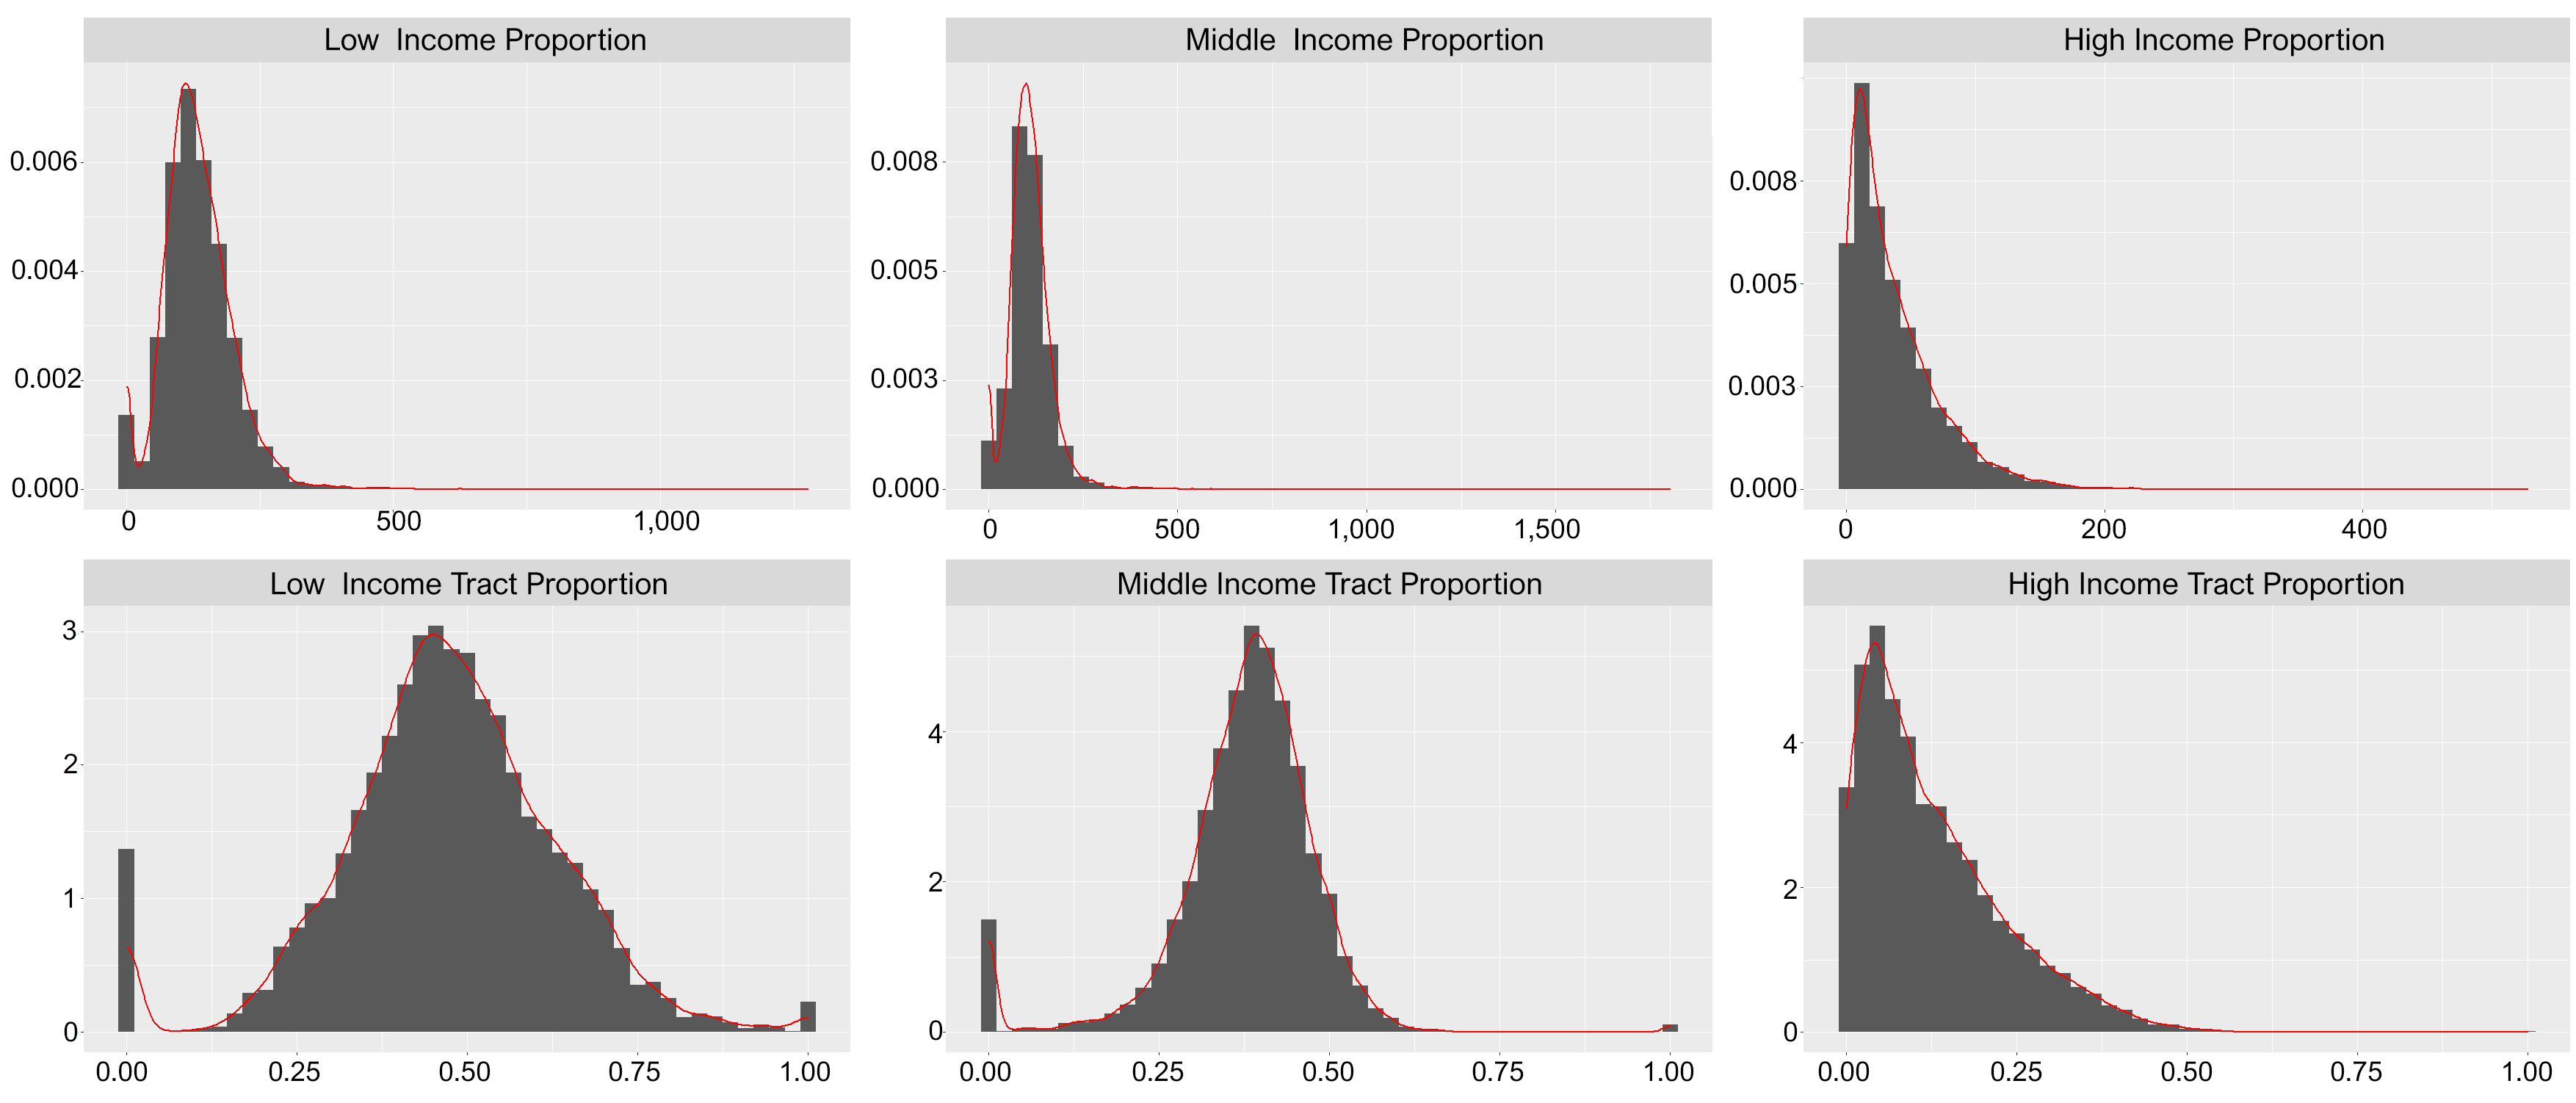
\includegraphics[width=1\textwidth]{body/figures/histograms_income.png}
    \caption{Caption}
    \label{fig:income_historgram}
\end{figure}

Income data for the 2016 census year was obtained at the SA1 level for the entirety of the GS metropolitan area. The dataset refers to the ABS' Total Personal Income dataset, INCP, which collects the gross personal income received each week by an individual \citep{abs_2017}. The data was filtered by an individual's place of usual residence to to reflect their residential locations. The INCP provided 17 income groups that ranged between \$0 to over \$3000 per week. These ranges were aggregated into three relative income groups, with income threshold adapted from \cite{acoss_2016} and \cite{p_aus_2019}. As such, low-income groups in this study are defined as individuals with a personal income of less than \$649 per week; middle-income groups ranged between \$650 to \$1,999 per week; and, high-income group were those with incomes above these thresholds. The distributions of these income ranges are illustrated in Figure \ref{fig:income_historgram}. Both the total income groups and and their relative census tract proportions are taken into consideration. A total of 1.5 million low-income-- ($\Bar{x}_{l\_tract} = 0.471$), 1.3 million middle-income-- ($\Bar{x}_{m\_tract} = 0.376$), and 0.4 million high-income-- ($\Bar{x}_{h\_tract} = 0.153$) individuals were enumerated in the dataset bringing the dataset size to ~3.2 million individuals.\\

\subsubsection{Journey to Work}

Commuting data was also obtained for the 2016 census year from the ABS. This refers particularly to the Journey to Work dataset, which includes the recorded number of individuals reporting to from a SA1-level 'Place of Usual Residence' to a Destination Zone (DZN) level 'Place of Work'. DZN areas are constructed from mesh block boundaries, but are not considered a statistical boundary \citep{abs_2016}. The dataset comprises reported population flows in the entire GS Metropolitan area. 11,171 SA1 and 2,233 DZN entries were noted in the dataset. Approximately, 1.21 million persons are enumerated within this data with respect to their individual flows, which equated to approximately 25 million individual trips between all origin and destination zones. A cursory inspection of the Journey to Work dataset reveals that the Sydney City Centre and its surrounding appears to be the central locus of employment, with approximately 25 per cent of all flows. Other loci of employment with relatively high densities of population flow include Parramatta, North Sydney, Campbelltown, and Gosford. The distribution of flows show less variation density variations across all other DZN areas. \\

\renewcommand{\baselinestretch}{0.8}
\begin{table}[!ht]
  \centering \small
    \begin{tabular}{c|ccccc|c}
    \textbf{O/D} & \textit{110286283} & \textit{110286284} & \textit{110296249} & \textit{\ldots} & \textit{116090001} & \multicolumn{1}{l}{\textbf{Origin Sum}} \\
    \midrule
    \textit{1102801} & 0     & 0     & 0     & \ldots & 0     & \textit{0} \\
    \textit{1102802} & 3     & 55    & 5     & \ldots & 0     & \textit{215} \\
    \textit{1102803} & 0     & 58    & 0     & \ldots & 0     & \textit{194} \\
    \textit{1102804} & 0     & 15    & 0     & \ldots & 0     & \textit{57} \\
    \textit{1102805} & 6     & 27    & 0     & \ldots & 0     & \textit{104} \\
    \vdots & \vdots & \vdots & \vdots & $\ddots$ & \vdots & \vdots \\
    \textit{1160910} & 0     & 0     & 0     & \ldots & 24    & \textit{178} \\
    \midrule
    \textbf{Destination Sum} & \textit{259} & \textit{591} & \textit{403} & \ldots & \textit{187} & \textbf{2,428,260} \\
    \end{tabular}
    \caption{Add caption} \label{tod_flows}
\end{table}%

The Journey to Work dataset was further extended to obtain both origin and destination capacities; and, this can be derived from the sum of flows at both origin and destination zones (ref. Table \ref{tod_flows}). The derived variables here represent important components in this study's downstream accessibility analysis; and, their inputs within the developed model will be discussed in the subsequent section. The flow matrix was then restructured into a simple dataframe, which enabled the dataset to be joined by their respective zone codes to the appropriate SA1 and DZN boundary vectors. This data layer was segmented with proprietary vector data of house footprints obtained from Geoscape to identify the critical mass of houses within each delineated boundary. A median-weighted centroid was appended within each SA1 and DZN building cluster to obtain a single point for each origin-destination zone (ref. Figure \ref{fig:odpoints}).\\

\begin{figure}[!ht]
    \centering
    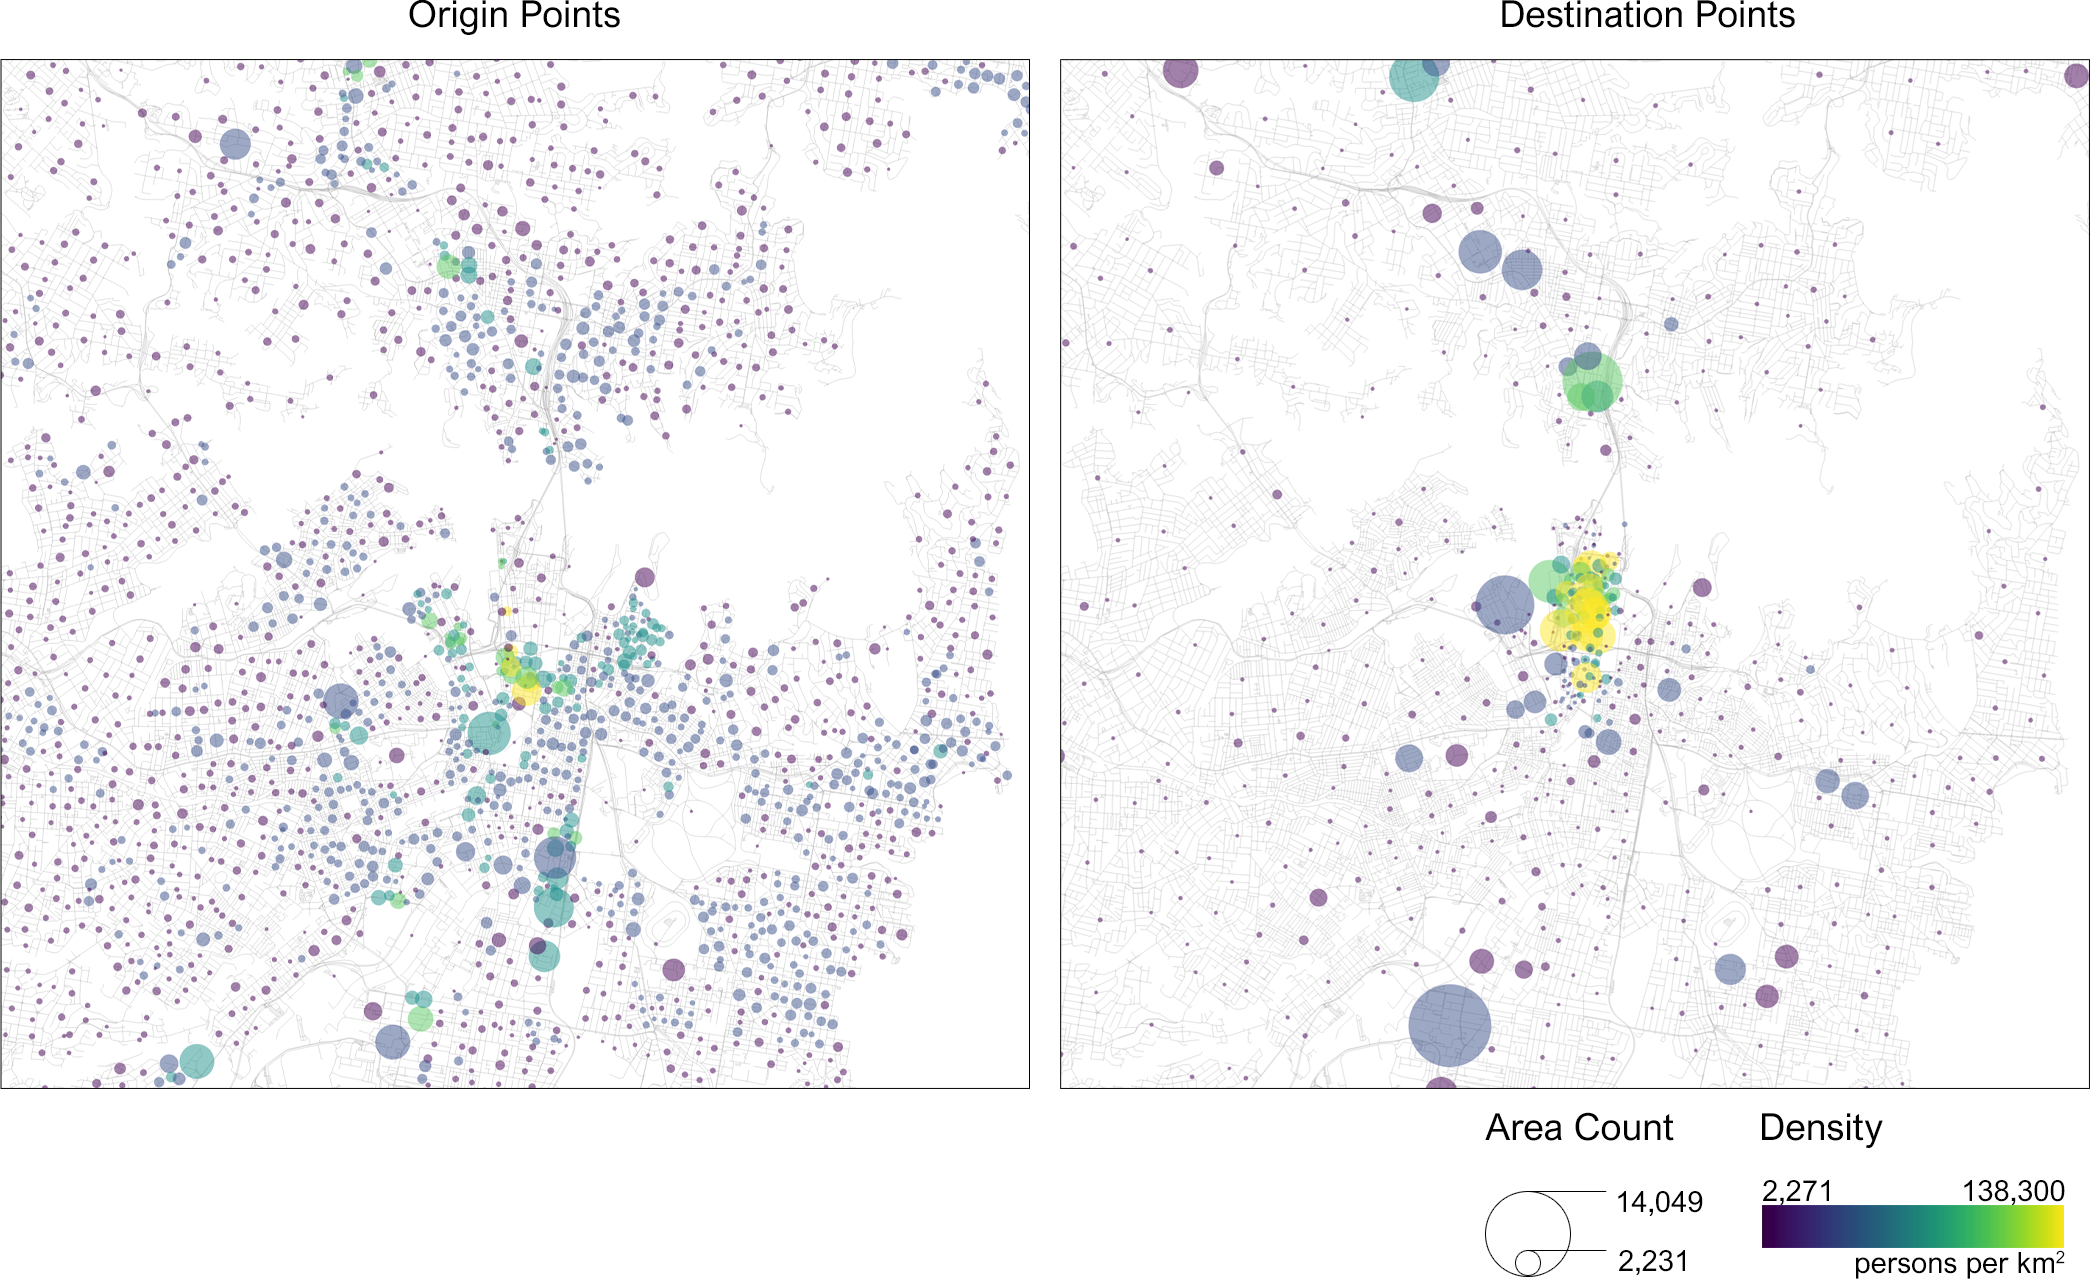
\includegraphics[width=1\textwidth]{body/figures/od_points.png}
    \caption{Caption}
    \label{fig:odpoints}
\end{figure}

\subsection{Road Network}

The transportation network for the GS Metropolitan area from the GeoFabrik\footnote{Site Available at $http://geofabrik.de/$} repository of OpenStreetMap (OSM) features on 5\textsuperscript{th} August 2020. All OSM data layers within the Australian sub-region was selected, which included a separate vector dataset of all transport lines in the region. The dataset was then processed in two stages to obtain a functional road network for GS. First, a spatial subset of the data was created with boundary files obtained from the ABS. The vector boundaries were filtered by their individual region code attribute, '\textit{1GSYD}', to return only data of the GS region. The full OSM transport network was clipped to this boundary to obtain all line features within GS area. Next, the trimmed GS transport network was then filtered through their attributes to obtain a network traversable by vehicles. These specific classes were defined from the metadata descriptions provided by \cite{topf_2009}. This process excluded line data for inappropriate transport modes such as bridleways, cycleways, and pedestrian only walkways. It should be noted that all unclassed transport links were also included in formation of the road network. The distribution of road type and the total road lengths can be found in Table \ref{tab:road}.\\

\renewcommand{\baselinestretch}{0.8}
\begin{table}[!ht]
    \centering \small
    \begin{tabular}{lrr}
    \textbf{Classification} & \multicolumn{1}{r}{\textbf{Line Count}} & \multicolumn{1}{r}{\textbf{Total Length (km)}} \\
        \midrule
        Motorway & 11,220 & 2,466.10 \\
        Primary & 10,305 & 1,755.28 \\
        Residential & 178,668 & 23,203.15 \\
        Secondary & 16,705 & 2,537.34\\
        Shared & 116   & 11.70 \\
        Tertiary & 23,495 & 3,140.60 \\
        Tracks & 10,286 & 6,529.46 \\
        Unclassed & 8,716  & 2,363.12 \\
        \midrule
        \textbf{Total} & \textbf{259,511} & \textbf{42,006.73}\\
    \end{tabular}
    \caption{Caption}
    \label{tab:road}
\end{table}

The obtained road network was then processed to correct for any  topological errors. This process involved the rectification of several error features, which included issues of excessive vertices, overlaps, self-intersections, pseudo-nodes, and disconnected road islands. In this study, all line intersections were accounted to obtain all possible edge features given the study's lack of ancillary data to correct for all possible continuous throughways. All errors arising from the above specification would be thus equally imposed throughout the entire network. To ensure the full connectivity of the obtained road network, a reiterative intersection detection algorithm was developed and implemented to obtain all possible edge connections. In this algorithm, all 'motorway' features were used to reiteratively select all road intersections up to the boundaries of GS. All unselected (i.e., disconnected road islands) clusters were discarded from the subsequent analysis. Figure \ref{fig:cleaned_road} illustrates a small sub-region of the cleaned network.\\

\begin{figure}[!ht]
    \centering
    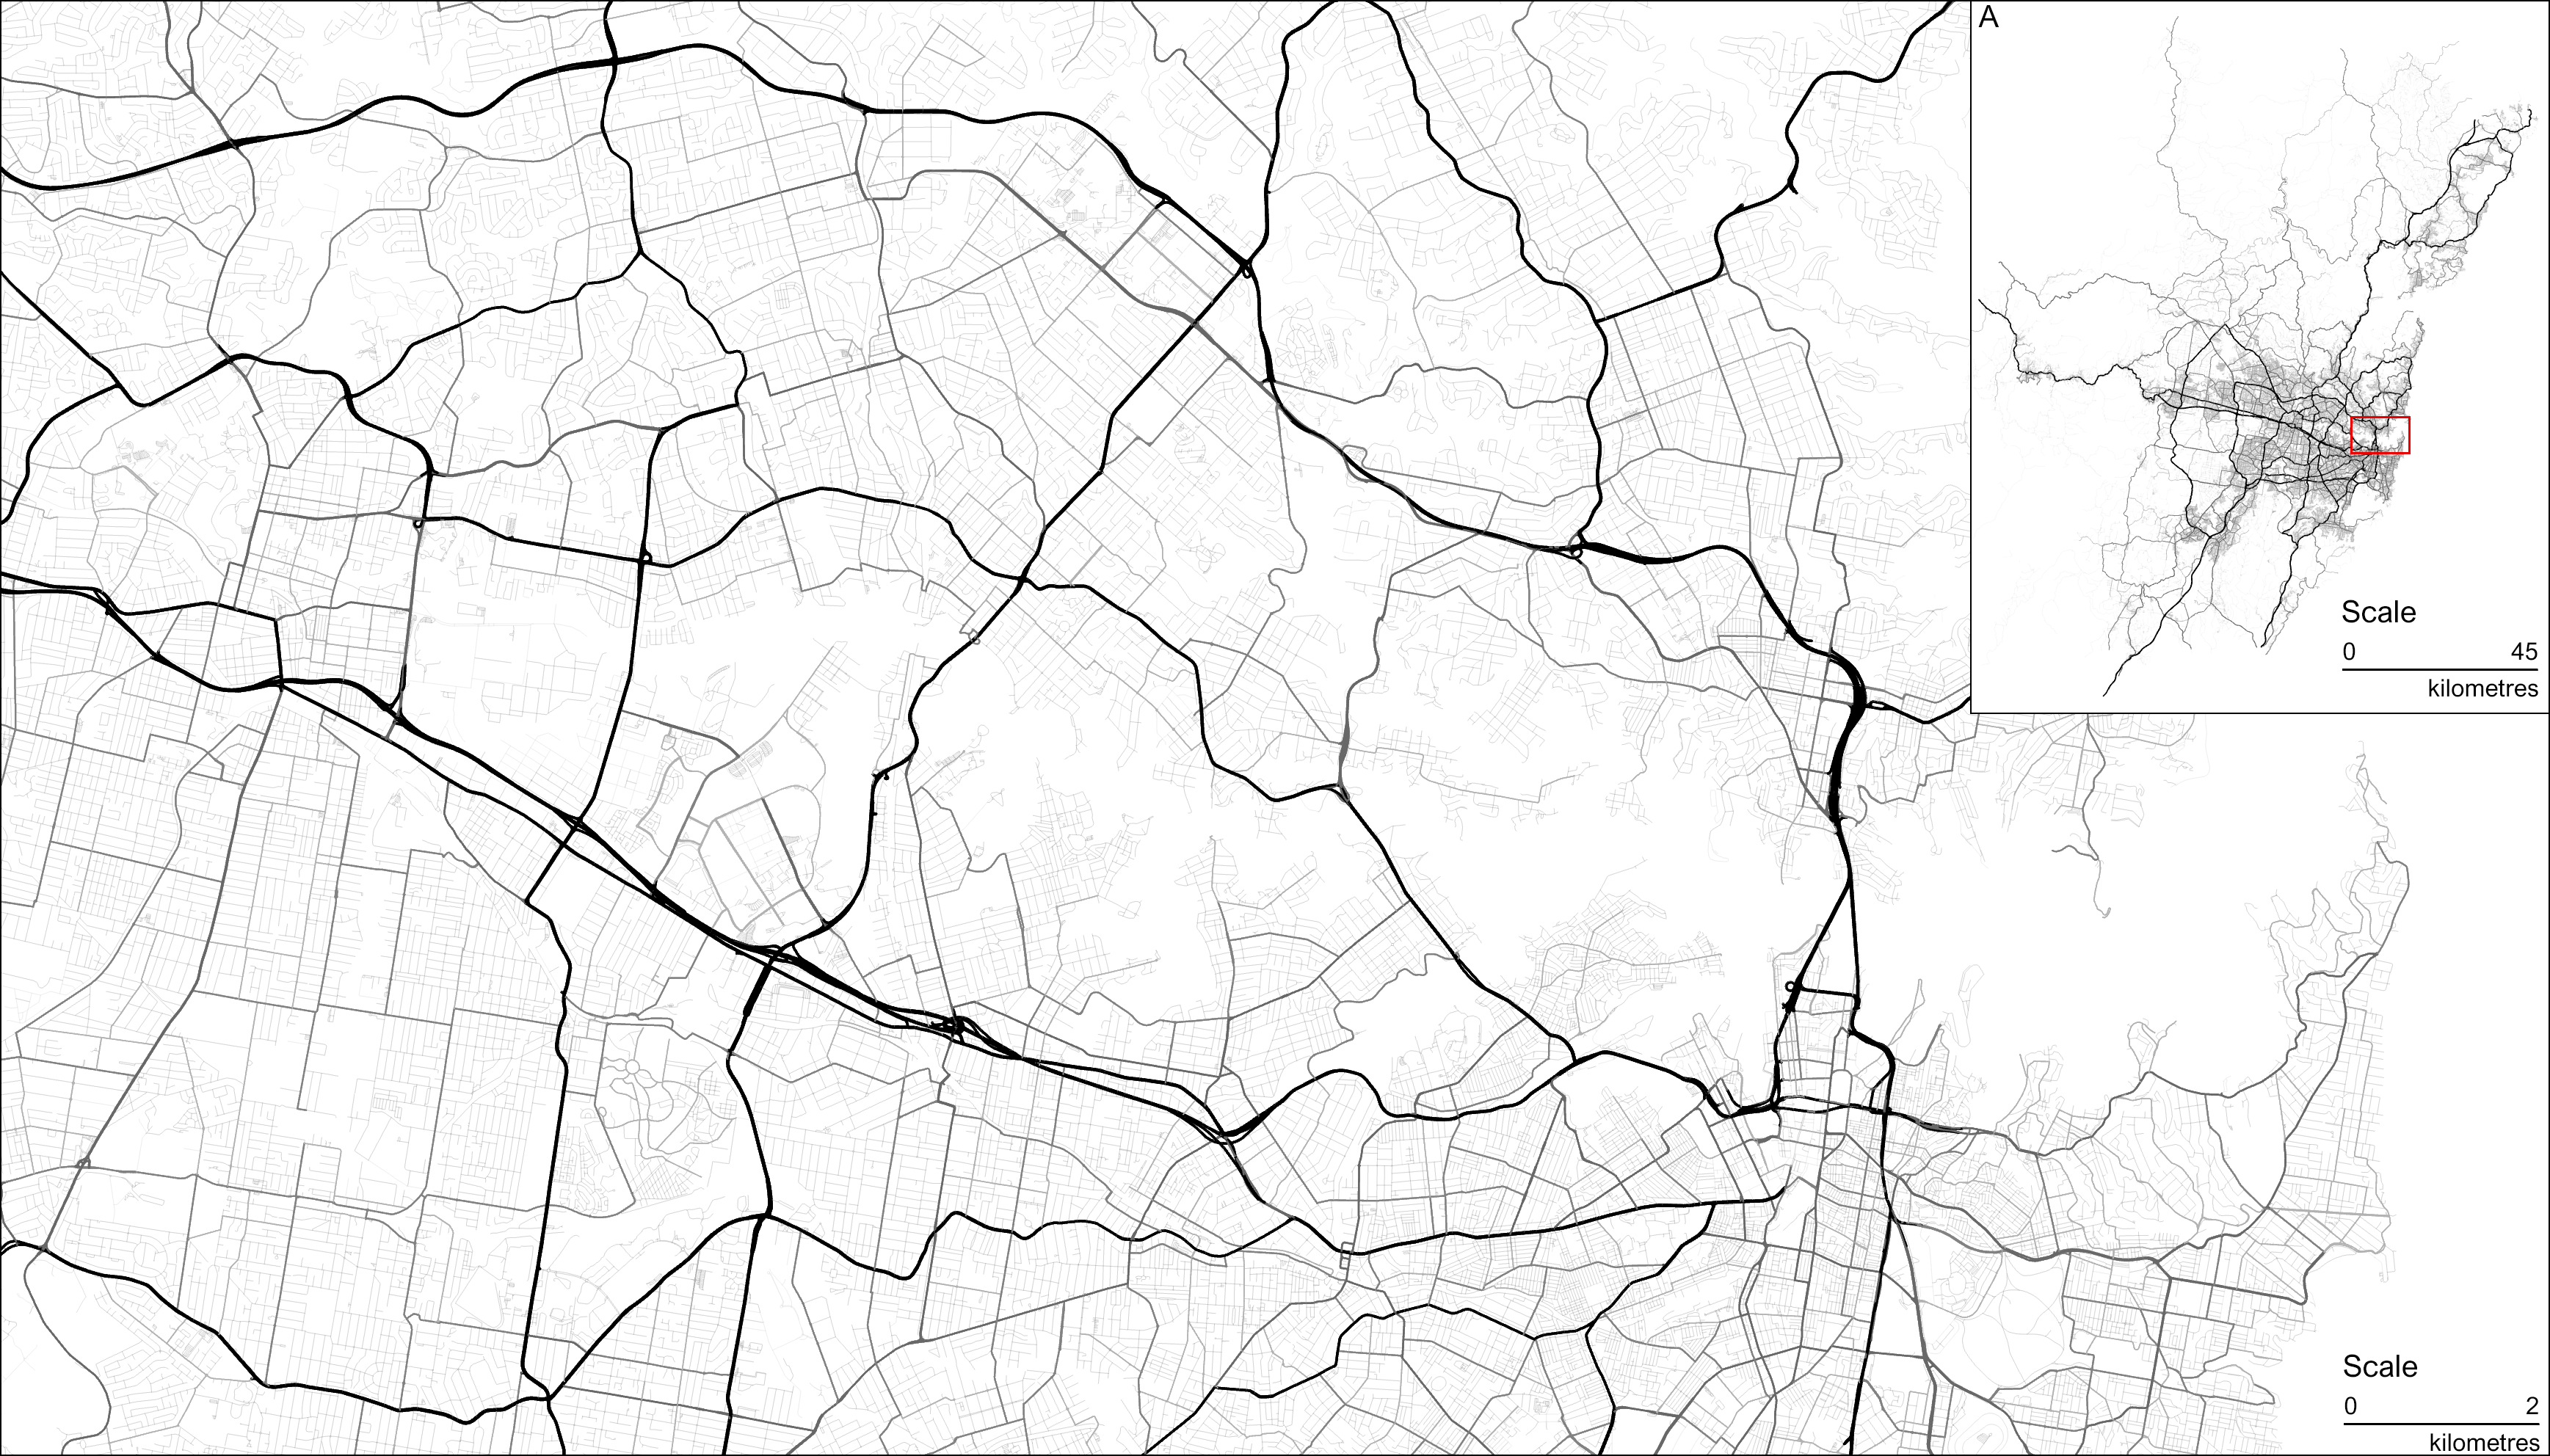
\includegraphics[width=0.95\textwidth]{body/figures/road.png}
    \caption{Caption}
    \label{fig:cleaned_road}
\end{figure}

The processed road network was subsequently used to calculate the separating network distance between each origin and destination point. This quantification represents the next major component to derive GS's accessibility score. A network-based distance calculation was preferred over Euclidean distances due to the anisotropic nature of the built-environment. This particularly pertinent for GS --- in which, its physical environment encompasses significant topological features that separate proximate areas. Figure \ref{fig:flows} illustrates this point succinctly, with the water bodies of Sailors Bay and Peach Tree Bay viewed as strong separating features. It highlights the need to consider more realistic environmental features; and, in particular, their effect in augmenting the separation between origin-destinations points through transport network availability.\\

\begin{figure}[H]
    \centering
    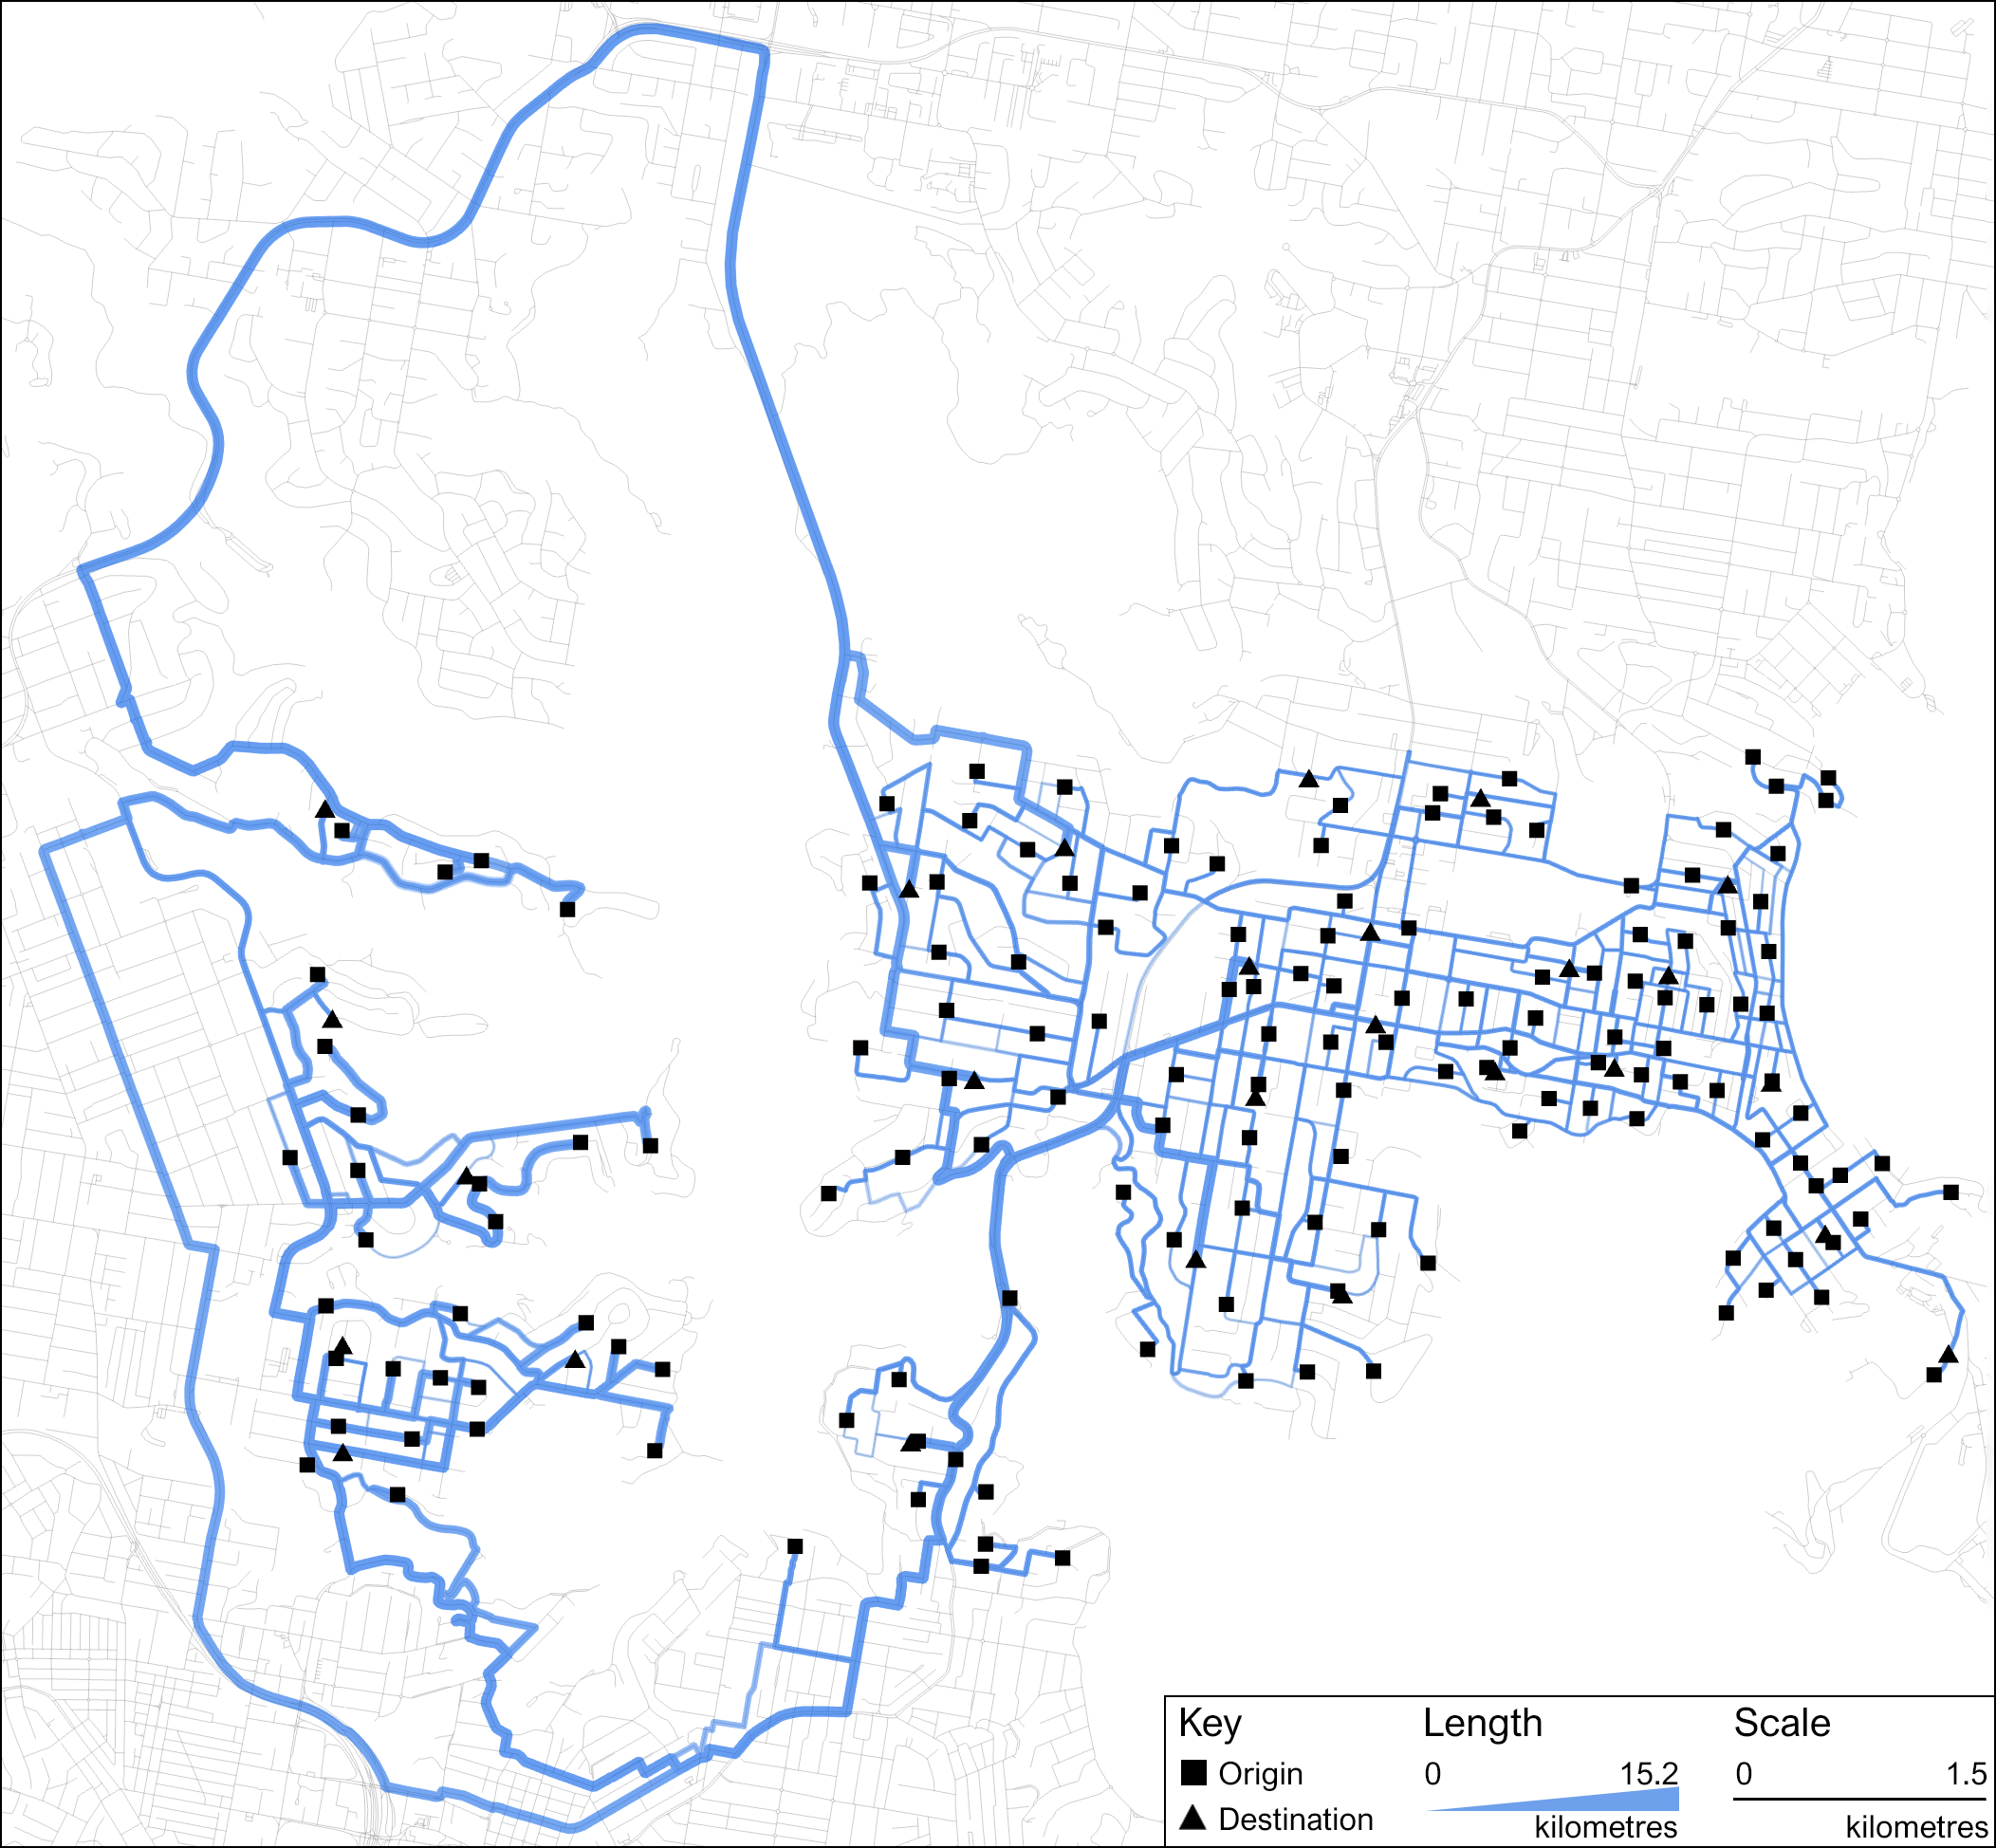
\includegraphics[width=0.65\textwidth]{body/figures/OD1.png}
    \caption{Caption}
    \label{fig:flows}
\end{figure}

\subsection{House Price}

The house price data used in this study was obtained from the Australian Property Monitor (APM) dataset from the Australian Urban Research Infrastructure Network (AURIN). The data is comprised of over property sales between 1994 and 2020. The dataset set includes large number of individual variables for each property, with key information on the physical characteristics, temporal distribution of sales, and contract sale prices being particularly relevant to this study. A relatively smaller subset of the APM data was only made available to the present study. This is comprised of approximately 1.82 million property sales ranging between 2006 and 2020 These sales data included both house and unit sales --- from which, only houses were filtered out. Figure \ref{fig:house_price} illustrates the change and relative frequency sales and sale prices for houses over the the above time range. As this paper aims to provide a synoptic analysis in GS, a subset of the house prices transacted in the two quarters of 2016 was used, which included 32,068 house price data points. This date range was chosen with the utilised census data in mind.\\

\begin{figure}[!ht]
    \centering
    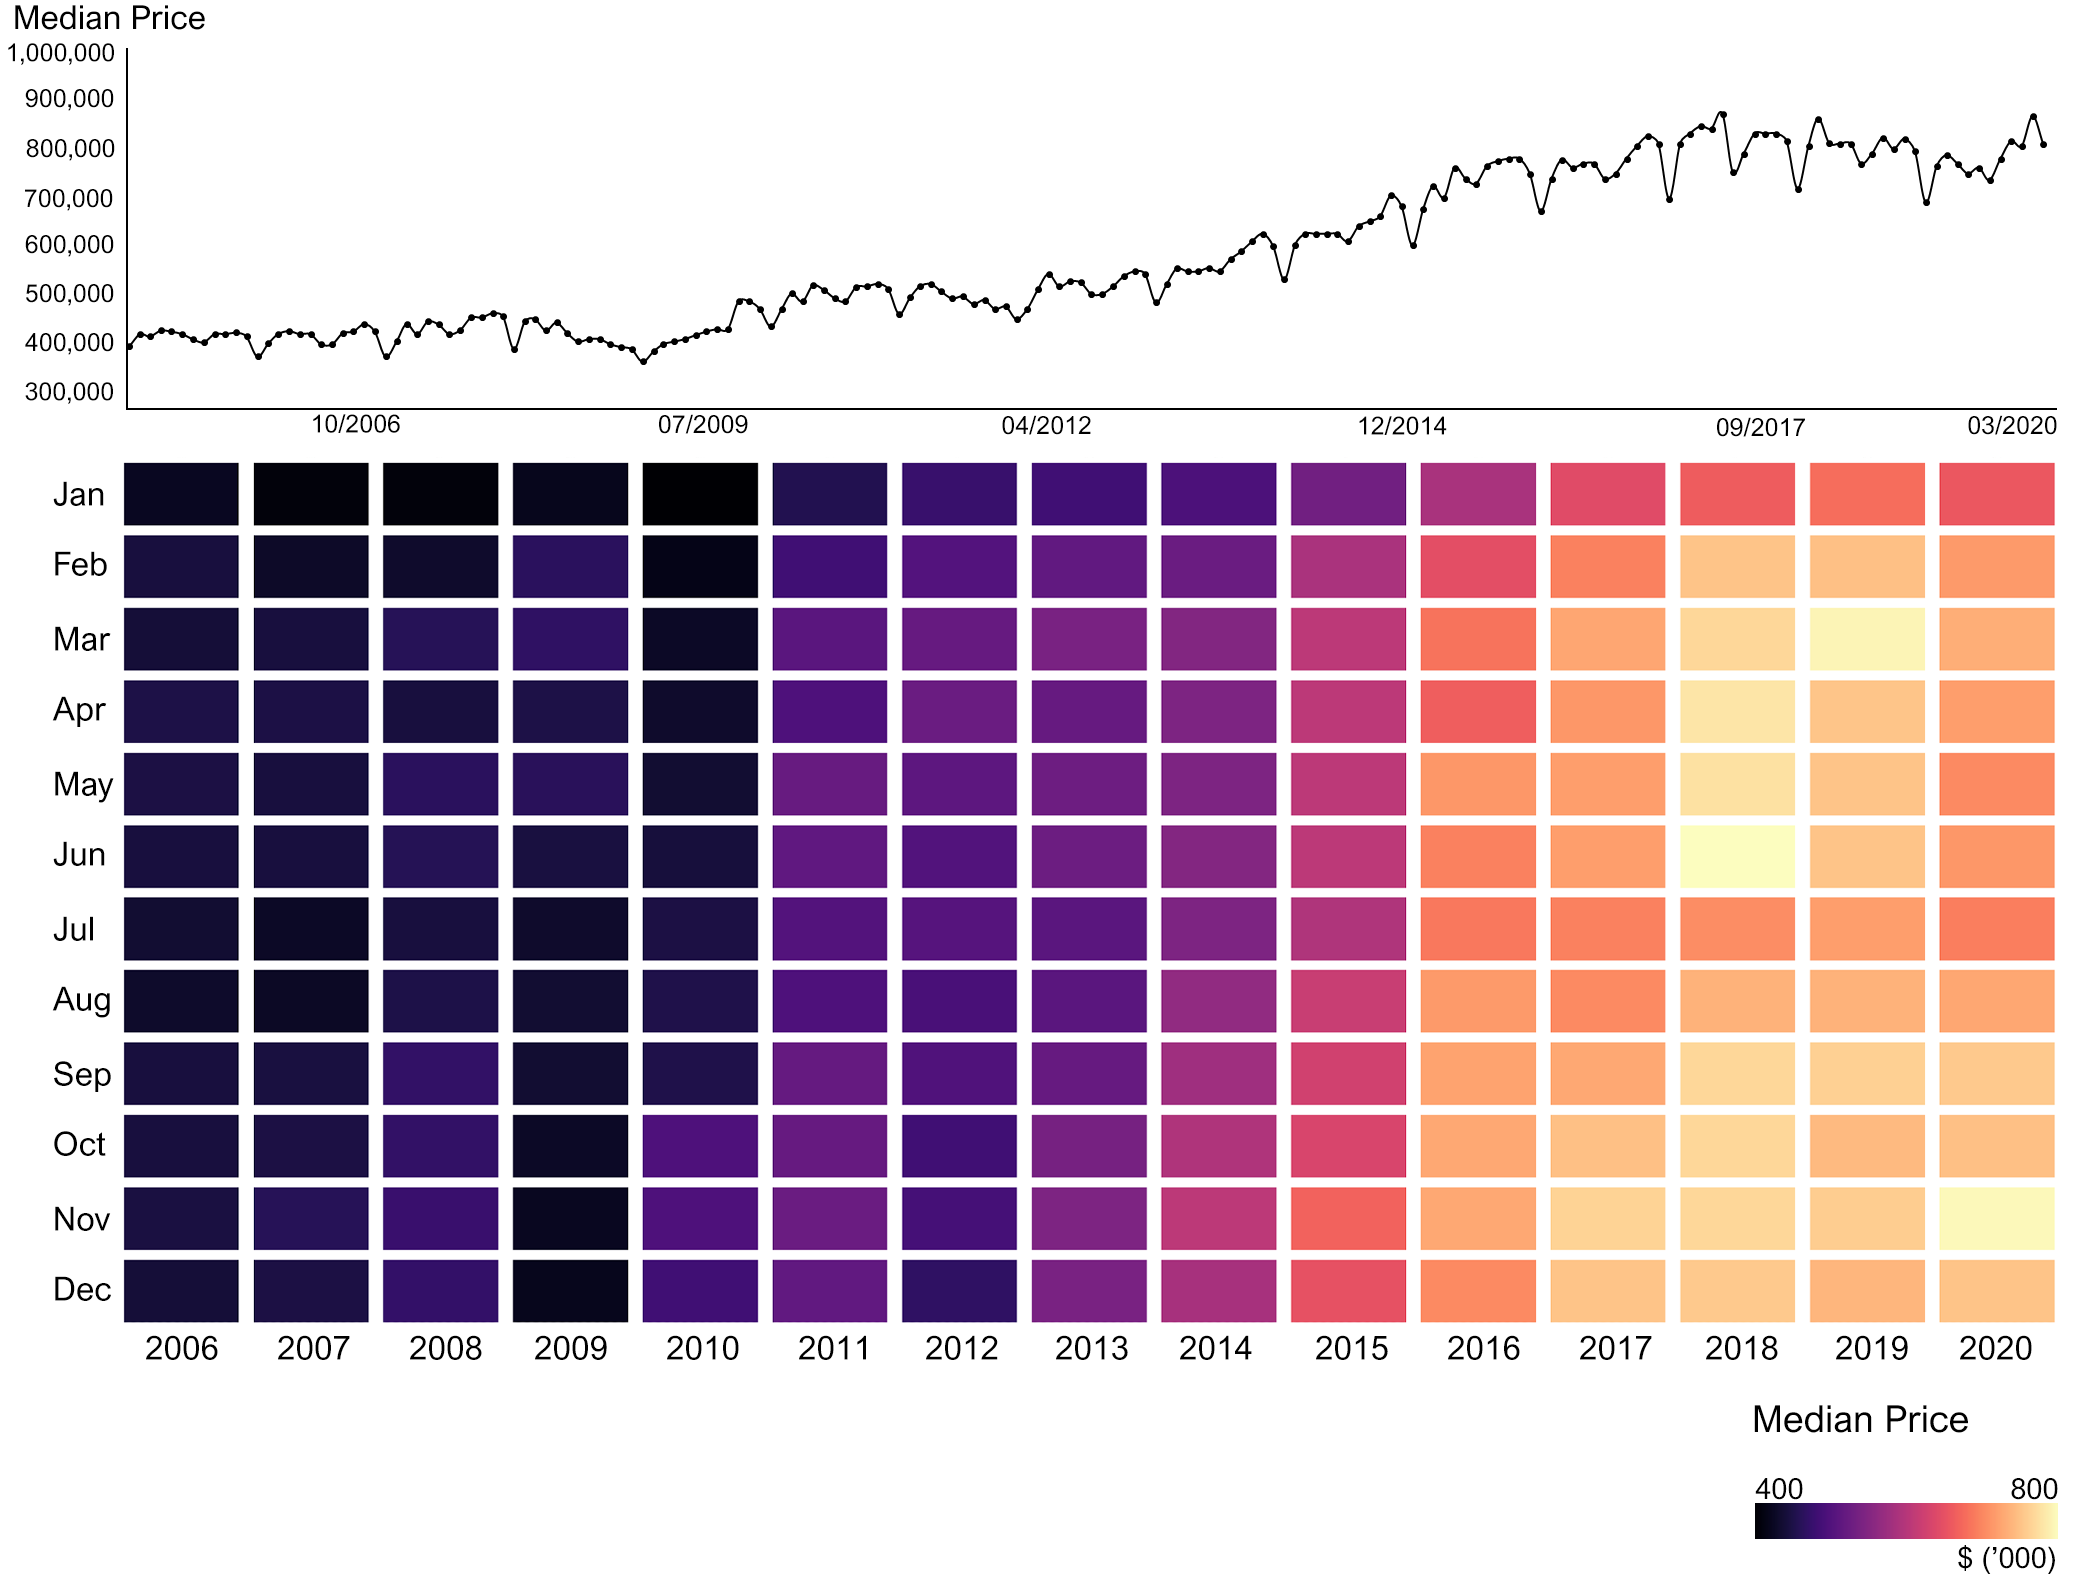
\includegraphics[width=0.95\textwidth]{body/figures/house_price_data.png}
    \caption{Caption}
    \label{fig:house_price}
\end{figure}

The dataset was then processed in several rungs to negate issues of zero-inflation downstream; and, to also remove price outliers. Outliers in this study are defined as those prices that are $\leq 2.5$ per cent and $\geq 97.5$ per cent within the house price range. All property entries were then geocoded using the Geocoded National Address File (G-NAF) available through PSMA Australia.\\ %The transaction density at the SA1 level is visualised in Figure \ref{fig:sold_prop}. It is worth reiterating that the dataset includes only properties characterised as 'houses', which excludes zones where no landed dwellings are found.\\

%\begin{figure}[!ht]
%    \centering
%    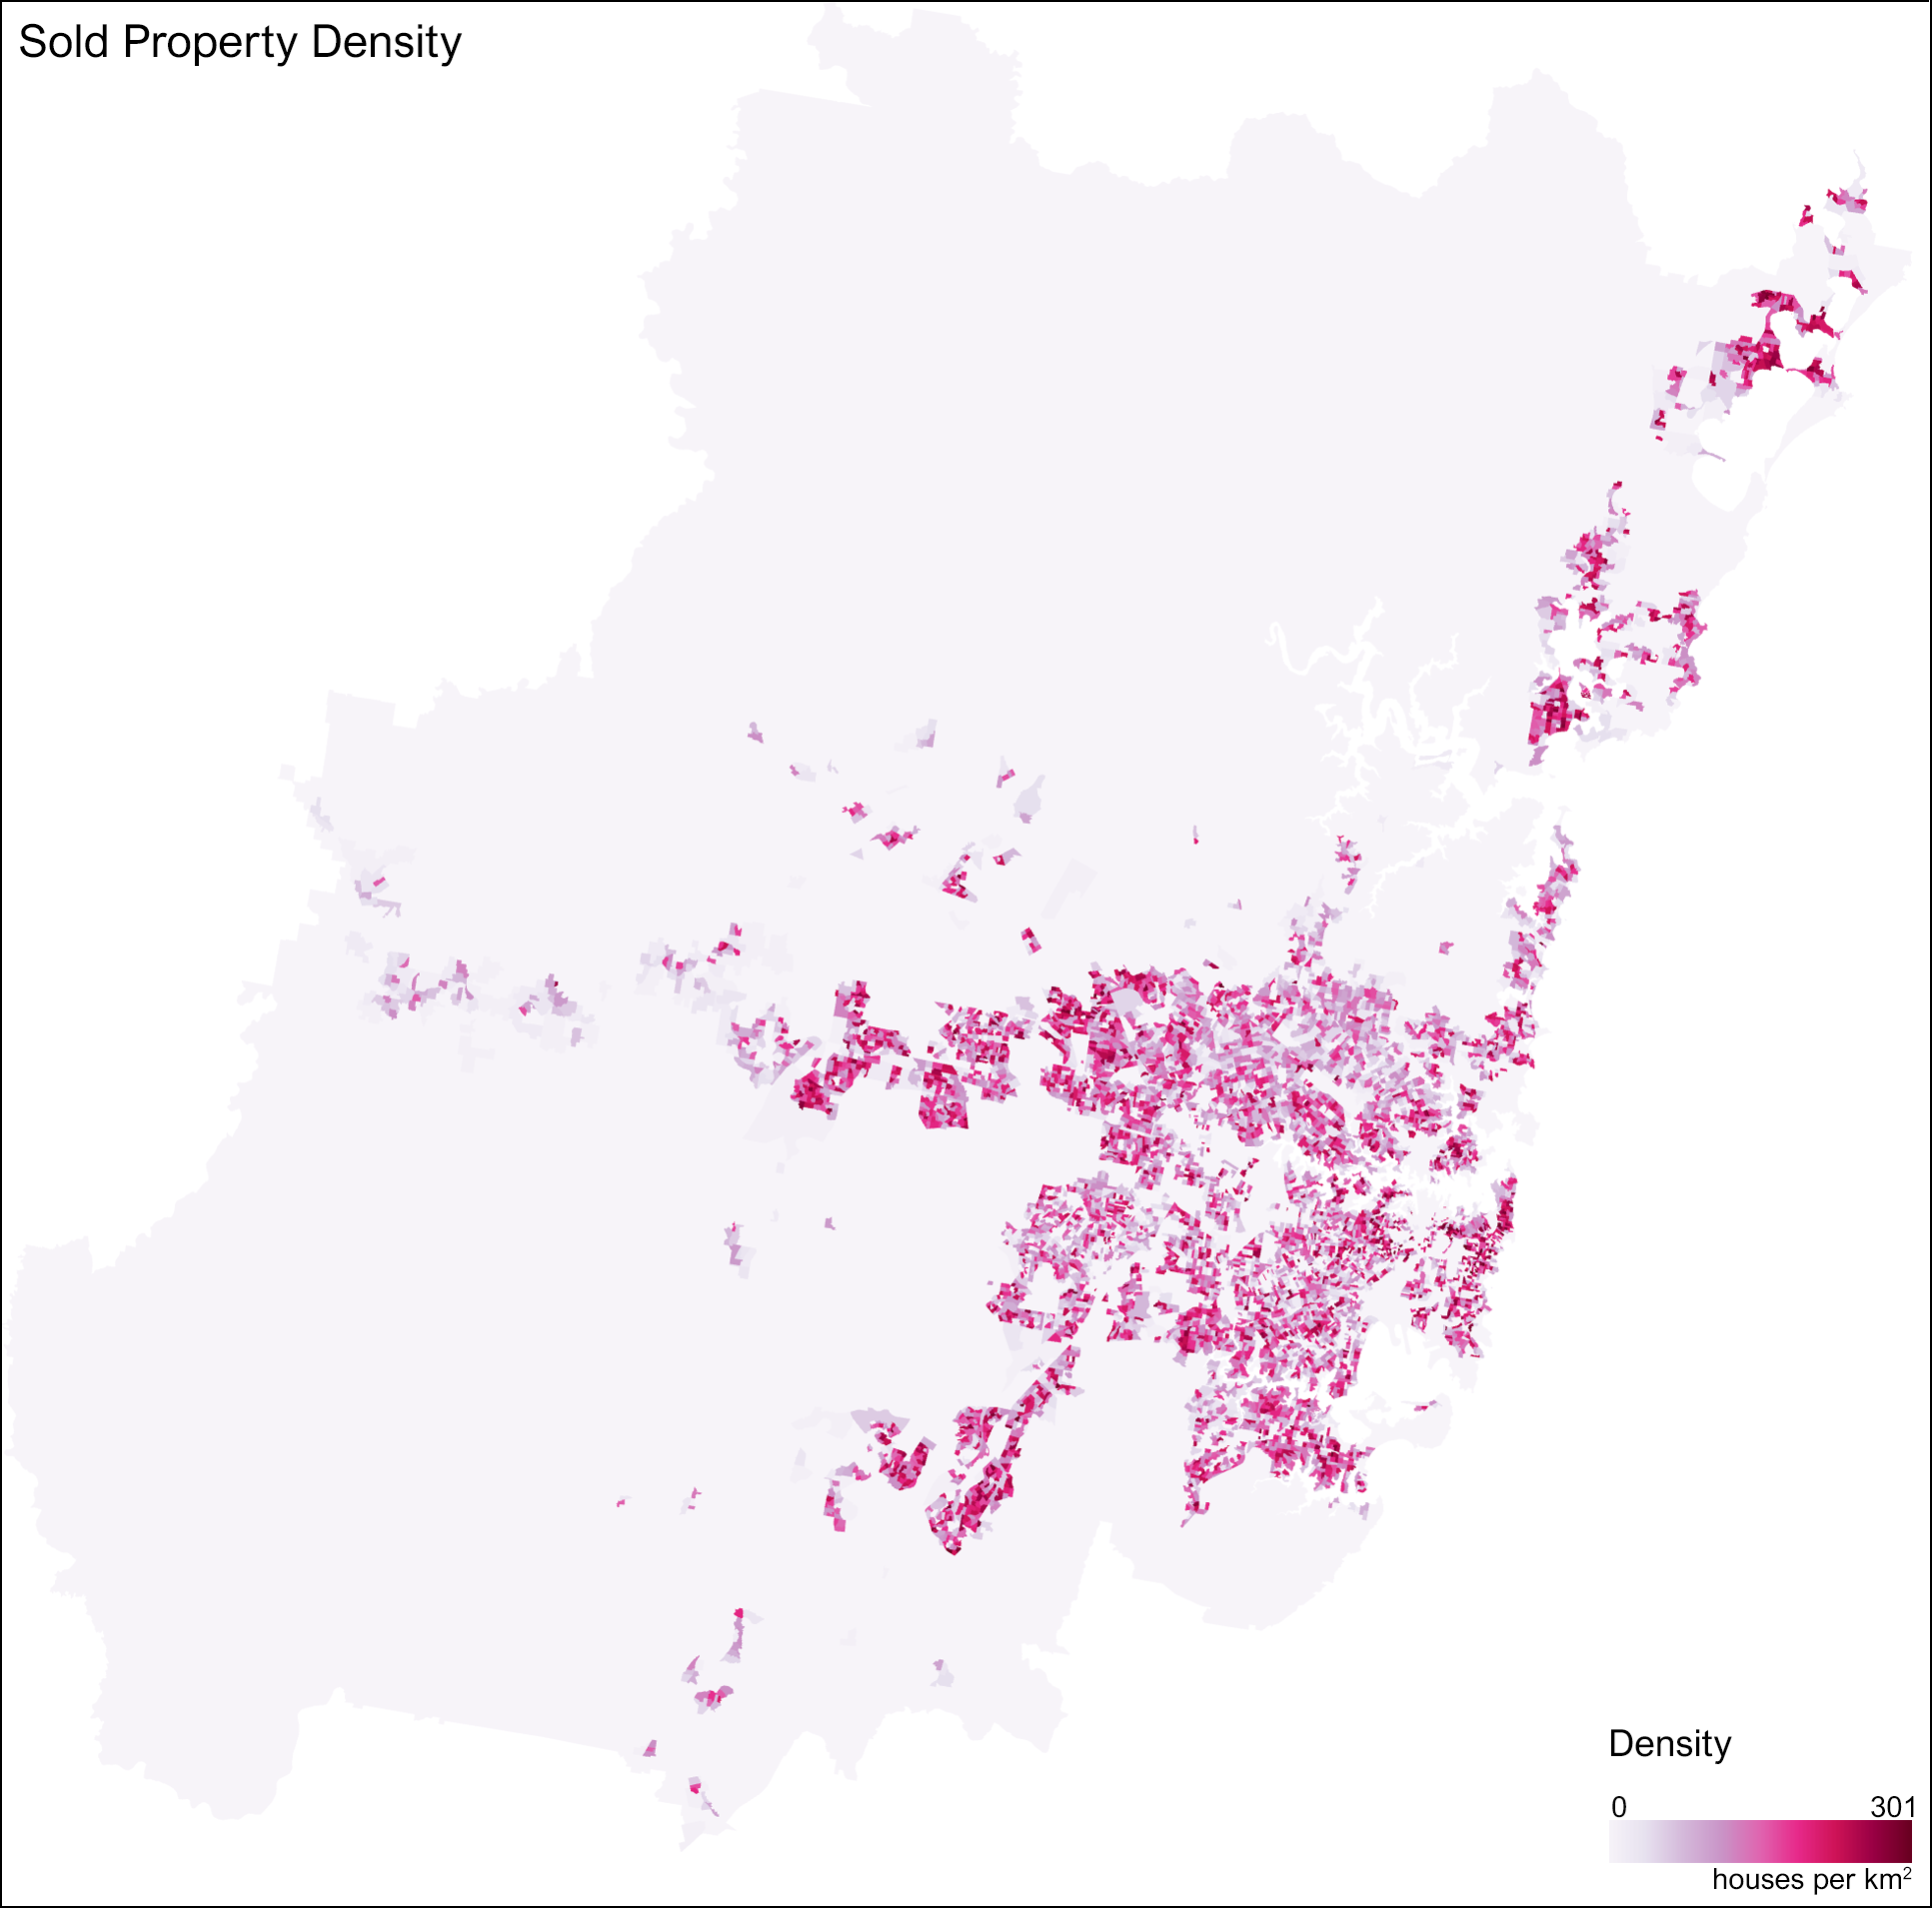
\includegraphics[width=0.7\textwidth]{body/figures/sold_prop_density.png}
%    \caption{Caption}
%    \label{fig:sold_prop}
%\end{figure}

\subsection{Points of Interest Data}

A large dataset of urban amenities was also made available to this study from PSMA Australia. This included the centroid locations of major transport hubs (e.g., bus interchanges, airports, train stations), education facilities (e.g., primary schools, secondary schools, universities), and urban services (e.g., police stations, hospitals, shopping centres, libraries, museums). The shortest path distance was calculated between all properties within the data subset to each of the closest points of interest (PoI). A full list of the considered PoI features utilised in this study is listed in Table \ref{tab:pois}.\\

\textbf{** REDO TABLE TO ADD ALL OTHER POIS}

\renewcommand{\baselinestretch}{0.8}
\begin{table}[!ht]
  \centering \small
    \begin{tabular}{lrrlr}
    \textbf{Feature} & \multicolumn{1}{l}{\textbf{Count}} &       & \textbf{Feature} & \multicolumn{1}{l}{\textbf{Count}} \\
\cmidrule{1-2}\cmidrule{4-5}    Airport & 102   &       & Museums & 282 \\
    Beach & 647   &       & Parks & 13,089 \\
    Sydney City Centre & 1     &       & Police Stations & 450 \\
    Secondary City Centres & 29    &       & Rail Stations & 525 \\
    High Schools & 696   &       & Shopping Centres & 488 \\
    Hospitals & 213   &       & Sports Centres & 2365 \\
    Libraries & 418   &       & Swimming Pools & 564 \\
    Light Rail Stations & 23    &       & Universities & 70 \\
\cmidrule{1-2}\cmidrule{4-5}    
\end{tabular}%
  \label{tab:pois}%
    \caption{Add caption}
\end{table}%

\section{Methods}
\label{sec:method}

\subsection{Entropy Measures}
Entropy values are powerful and widely used as a statistical measure to describe specific attribute compositions within the urban system \citep{batty2014entropy}. They are classically used to quantify disorder in an area; in which, high entropy values equate to large variances that are inherent within that area \citep{batty2014entropy, wilson2013entropy}. Neighbourhood entropy are robust indicators of spatial variance; and, it is widely applied in land-use analyses, population composition, and economic activity \citep{tan2003laws, wilson2013entropy}. It is also considered within segregation analyses given its reflection of the heterogeneity of populations in localised areas \citep{fischer2003relative}. Following this logic, they offer a means to better understand diversity within a system. Here, the basic statistical form of entropy is adopted, and its application to income groups are implemented in this study. \\

The entropy measure utilised in this study can be considered by Equation \ref{entropy_eqn},

\begin{equation}
    H_{i} = - \sum^{k}_{j=1}P_{ij} \cdot ln(P_{ij})
    \label{entropy_eqn}
\end{equation}

\ldots where, entropy ($H$) at location $i$, is determined by the  proportion of a specific income group, $j$. $K$ in the above equation refers to the number of income group types within the model. The proportion of this income group, $P_{ij}$, can be calculated with Equation \ref{eqn_porportion},

\begin{equation}
    P_{ij} = \frac{N_{ij}}{\sum_{j=1}^{k}N_{i}}
    \label{eqn_porportion}
\end{equation}

\ldots with, the tract total of an income group, $j$ in $N_{ij}$, is considered against the total of all income groups in the same tract, $N_{i}$. The maximum value of entropy ($H_{max}$) within a system is quantified with the following equation (ref. Equation \ref{hmax}).

\begin{equation}
    H_{max} = ln(k)
    \label{hmax}
\end{equation}

\subsection{Accessibility Indices}

As indicated in the discussion above, there are several established methodologies to determine accessibility within the urban system. This paper will consider accessibility as estimates derived from the gravity model expressed previously in Equation \ref{gravity}. It can be argued that, in this instance, the gravity potential model provides a more nuanced proxy of accessibility in GS, given the available population and flow data from the ABS. The models parameters and coefficients are computed in line with these datasets in the following way.\\

From the notation expressed in Equation \ref{gravity}, the gravity potential model can be alternatively written as, Equation \ref{wilson_grav}, 

\begin{equation}
    T_{ij} = k V_{i}^{\mu} W_{j}^{\alpha} d_{ij}^{\beta}
    \label{wilson_grav}
\end{equation}

\ldots where, the flows ($T_{ij}$) are derived in the same way from mass term and attraction factors noted at the origin ($V_{i}^{\mu}$) and destination ($W_{j}^{\alpha}$). It is worth reiterating that, the model is implemented using the JTW flows as $T_{ij}$; the total DZN density as $W_{j}^{\alpha}$; and, the origin population total as $V_{i}^{\mu}$. Following \citeauthor{dennett2012estimating}'s (\citeyear{dennett2012estimating}) work, the natural log of each component within the model can thus be taken and respecified into in a log-linear format (ref. Equation \ref{wilson_grav_log}):

\begin{equation}
    ln T_{ij} = k + \mu ln(V_{i}) + \alpha ln(W_{j}) - \beta ln(d_{ij})
    \label{wilson_grav_log}
\end{equation}

\ldots whereby, the model is considered as 'saturated' with all possible components to estimate potential flows. With this, the model can be fitted simultaneously to derive the necessary coefficients and factors for the relative attraction and emissivity of the origin and destination. However, considering the current specification, this study also implements a single production constraint (ref. Equation \ref{eqn:procon}) to converge the model estimates to converge the model accordingly to the origin totals ($O_{i}$) as seen in Equation \ref{prod_flow_cons},

\begin{equation}
    \sum_{j}T_{ij} = O_{i}
    \label{prod_flow_cons}
\end{equation}

Consequently, this allows the accessibility model to be reshaped into the Equation \ref{prod_constrained_mod},

\begin{equation}
    \delta_{ij} = exp(\sigma_{i} + \alpha ln W_{j} - \beta ln d_{ij})
    \label{prod_constrained_mod}
\end{equation}

\ldots where,  $\delta _{ij}$ refers to the observed flows; and, $\sigma_{i}$ is taken as a categorical predictor for all flows in each origin SA1 (i.e., each individual SA1 code). Having now appropriately specified the model, the parameters for $\alpha$ and $\beta$ are solved for. The final parameter values used are 0.121 and -2.278, respectively. With obtained parameters, the production-constrained model can be calculated as denoted by \cite{wilson1971family} with the appropriate balancing factor, $A_{i}$ (ref. Equation \ref{eqn:balancing_factors}). The preference for singly-constrained model over the attraction-production constraints is due to the unknown 'capacity' of employment within each DZN area; which, if constrained, would have been arbitrary. The calibration of the above parameters allows accessibility scores to computed with the classical gravity potential model (ref. Equation \ref{gravity}). The obtained values are then standardised between 1 and 0 for ease of interpretation. \\

The model performance is evaluated with the computed flow estimates against the observed flows. An acceptable $R^2$ of 0.61 was achieved, which suggests that the model is able to capture just over two-thirds of the employment flows occurring within GS. It is also worth noting that the above models utilise a power law as its distance-decay function ($f(d_{ij}) = d_{ij} ^{\beta}$) over its exponential counterpart ($f(d_{ij}) = exp^{d_{ij}{\beta}}$). Both functions were previously tested against the JTW observed flows; hence, the choice of the power-law function given its better results. \\

\subsection{Relationship Testing}

Having now considered the above data and models above, this study opts to conduct both an Ordinary Least Squares (OLS) regression and a Geographically Weighted Regression (GWR) to better understand their intrinsic relationships within the urban system. The OLS method is a global fitting method, which computes a single parameter estimates for each independent variable. However, given the spatial nature of the house price, income, and accessibility data, these relationships should also be tested with respect to their possible spatial variations. The model is derived from the traditional linear regression models; however, in its extension, the GWR includes a bandwidth parameter that considers a kernel of neighbouring points for each observation. Generally, the GWR model can be expressed as Equation \ref{GWR},

\begin{equation}
    y_{i} = \beta_{0}(u_{i},v_{i}) + \sum_{j}\beta_{k}(u_{i},v_{i})x_{ik} + \varepsilon_{i}
    \label{GWR}
\end{equation}

\ldots where the relationship between the dependent variable, $y_{i}$, and the set of independent variables, $j$, is represented by a continuous function $\beta_{k}(u_{i},v_{i})$ at different locations of ($u_{i}$, $v_{i}$) at observation $i$. Here, the location of each data point is represented by coordinates ($u_{i}$, $v_{i}$); $\varepsilon_{i}$ represents the residual variable of the model. The GWR requires a bandwidth parameter, $b$, to be set, which are either fixed or adaptive (i.e., variable values of $b$) kernels. A spatial weights matrix is then constructed, with points closer to location $(u_{i},v_{i})$ assigned a higher value, and those exceeding the $b$ parameter are nullified. This can be generally expressed by Equation \ref{weights},

\begin{equation}
w_{ij}= \begin{cases}
1, & \text{if } d_{ij} < b \\ 
0, & \text{otherwise} 
\end{cases}
\label{weights}
\end{equation}

\ldots where, $w_{ij}$ denotes the individual weights for each location of $(u_{i},v_{i})$; and, $d_{ij}$ representing the distance threshold in consideration. It should be noted that the general expression for the above weights matrix is often altered through a weighting function, which is typically a gaussian or bi-square function \citep{fotheringham2003geographically}. In this paper, an adaptive bi-square was opted for due to its more sensitive allocation of weights with the increasing distances of all other data points \citep{fotheringham2003geographically,fotheringham2016geographically, oshan2019comment}. This function is denoted by Equation \ref{weights_bi}:

\begin{equation}
w_{ij}= \begin{cases}
\left (1 - (\frac{d_{ij}}{b_{i(k)}})^{2}  \right )^{2}, & \text{if } \; d_{ij} < b_{i(k)} \\ 
0, & \text{otherwise} 
\end{cases}
\label{weights_bi}
\end{equation}

In comparison to the general weights function where the $b$ represents a single integer, the $b_{i(k)}$ parameter here is variable with $k$ representing the number closest to point $i$ \citep{albuquerque2017geographically}. The optimum bandwidths are finally chosen through the minimisation of the Akaike Information Criterion (AIC) \citep{fotheringham2003geographically,fabian2014method,albuquerque2017geographically}.\\

\subsubsection{Multicollinearity Diagnosis}

\begin{figure}[!ht]
    \centering \small
    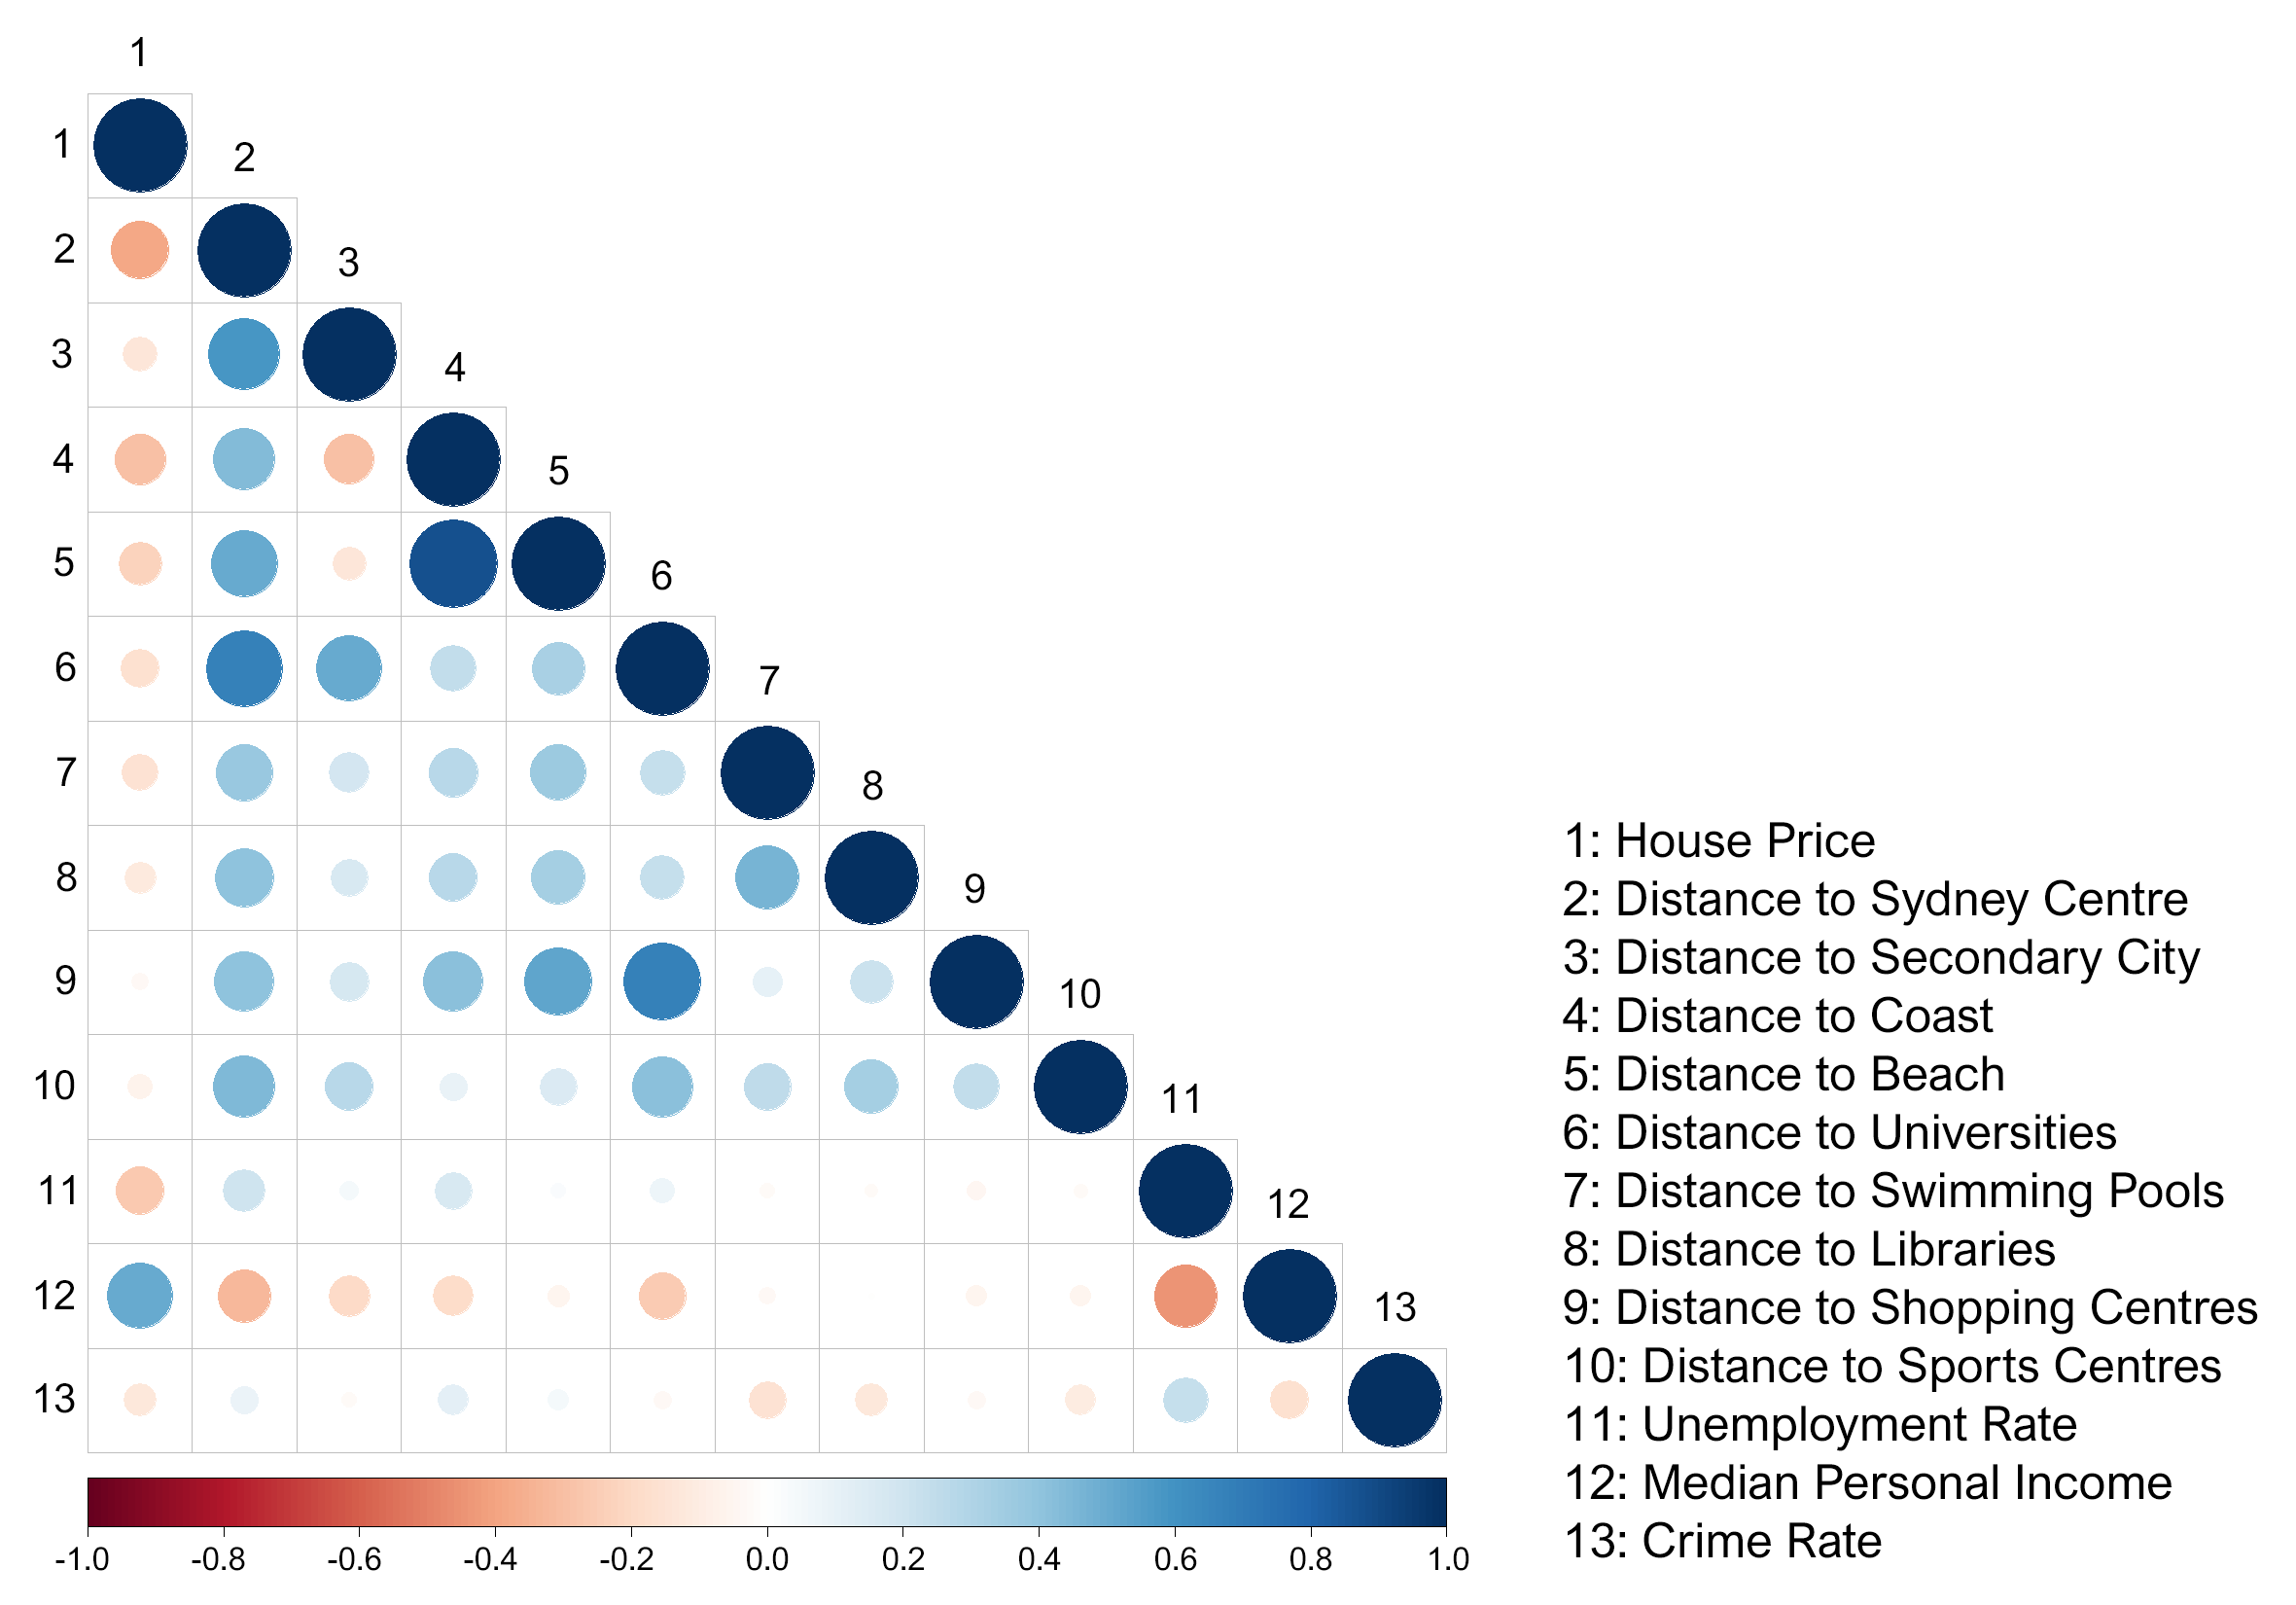
\includegraphics[width=0.65\textwidth]{body/figures/Entropy_CorrPlot2.png}
    \caption{Caption}
    \label{fig:collinear}
\end{figure}

\textbf{** REDO CORRPLOT}

The above house price dataset was then attributed to their respective neighbourhood-- and PoI datasets based on their location in GS. A test for multicollinearity was conducted to reduce the redundancy and imprecision in the regression model coefficient estimates arising from these variables (ref. Figure \ref{fig:collinear}). The diagnosis was approached by calculating the variance inflation factor (VIF) between each variable with respect to house prices. VIF accounts for the change in the independent variable coefficient estimate against any correlations between all independent variables within the model \citep{gareth2013introduction}.  \cite{gareth2013introduction} noted that a VIF that exceed 10 is often considered problematic. The tolerance factor, which is also included, considers the likelihood of each independent variable being unaccounted for by all other independent variables within th model. Remedial measures to address the arising issues with multicollinearity include variable exclusions, principal component analyses, or step-wise regression applications \citep{bruce2020practical}. This paper opted to exclude collinear variable pairs with an observed VIF scores greater than 10 ($VIF \geq 10$). The final variable subset and their respective VIF scores are detailed in Table \ref{tab:VIF_Score}.\\

\renewcommand{\baselinestretch}{0.8}
\begin{table}[H]
  \centering
    \small    \begin{tabular}{llll}
          & \textbf{VIF}   & \textbf{TOL}   & \textbf{Detection} \\
    \midrule
    Bedrooms & \multicolumn{1}{r}{1.1893} & \multicolumn{1}{r}{0.8408} & \multicolumn{1}{r}{0} \\
    Parking & \multicolumn{1}{r}{1.1334} & \multicolumn{1}{r}{0.8823} & \multicolumn{1}{r}{0} \\
    Distance to Sydney & \multicolumn{1}{r}{5.9793} & \multicolumn{1}{r}{0.1672} & \multicolumn{1}{r}{0} \\
    Distance to Secondary City & \multicolumn{1}{r}{3.4664} & \multicolumn{1}{r}{0.2885} & \multicolumn{1}{r}{0} \\
    Distance to Beach & \multicolumn{1}{r}{3.376} & \multicolumn{1}{r}{0.2962} & \multicolumn{1}{r}{0} \\
    Distance to Bus & \multicolumn{1}{r}{1.4894} & \multicolumn{1}{r}{0.6714} & \multicolumn{1}{r}{0} \\
    Distance to Highway & \multicolumn{1}{r}{2.6792} & \multicolumn{1}{r}{0.3732} & \multicolumn{1}{r}{0} \\
    Distance to Primary School & \multicolumn{1}{r}{1.2433} & \multicolumn{1}{r}{0.8043} & \multicolumn{1}{r}{0} \\
    Distance to University & \multicolumn{1}{r}{3.8986} & \multicolumn{1}{r}{0.2565} & \multicolumn{1}{r}{0} \\
    Distance to Swimming Pool & \multicolumn{1}{r}{1.5206} & \multicolumn{1}{r}{0.6576} & \multicolumn{1}{r}{0} \\
    Distance to Shopping Centre & \multicolumn{1}{r}{3.232} & \multicolumn{1}{r}{0.3094} & \multicolumn{1}{r}{0} \\
    Distance to Sport Centre & \multicolumn{1}{r}{1.4375} & \multicolumn{1}{r}{0.6957} & \multicolumn{1}{r}{0} \\
    Population Above 65 & \multicolumn{1}{r}{1.4889} & \multicolumn{1}{r}{0.6716} & \multicolumn{1}{r}{0} \\
    Crime Rate & \multicolumn{1}{r}{1.2346} & \multicolumn{1}{r}{0.81} & \multicolumn{1}{r}{0} \\
    \midrule
    Diagnostic Information: &       &       &  \\
    \multicolumn{4}{l}{\textit{Note: VIF Method failed to detect multicollinearity}} \\
    \multicolumn{4}{l}{\textit{0 = Collinearity is not detected by the test}} \\
    \end{tabular}%
    \caption{Add caption}
    \label{tab:VIF_Score}%
    \end{table}%

\section{Results and Discussions}
\label{sec:results}

\subsection{Income Distributions in Greater Sydney}

In response to this paper's first objective, the spatial distribution of income groups within the GS area was considered. Entropy statistics ($H$) were used as a measure to quantify the spatial diversity between these income. These values ranged from 0.00 to a maximum of 1.10 ($H_{max}$) --- whereby, in areas where $H = 1.10$, an equal distribution of all three income groups is observed. The global mean entropy value in GS was calculated to be 0.862, with a minimum and maximum of 0.00 and 1.09, respectively. \\

\renewcommand{\baselinestretch}{0.8}
\begin{table}[!ht]
  \centering \small
    \begin{tabular}{l|cccc}
          & \textbf{Low Income} & \textbf{Middle Income} & \textbf{High Income} & \textbf{Entropy} \\
    \midrule
    \textbf{Low Income} & 1.000 & -0.218 & -0.561 & -0.219 \\
    \textbf{Middle Income} & -0.218 & 1.000 & 0.198 & 0.565 \\
    \textbf{High Income} & -0.561 & 0.198 & 1.000 & 0.629 \\
    \textbf{Entropy} & -0.219 & 0.565 & 0.629 & 1.000 \\
    \end{tabular}%
      \caption{Add caption}
  \label{tab:entropy_incomes}%
\end{table}%

Table \ref{tab:entropy_incomes} quantifies the correlation coefficients between all income groups and their respective entropy values. What is first noticeable is the negative relationship between the distribution of low-income groups in Sydney with its middle-- ($R=-0.22$) and high-- ($R=-0.56$) income counterparts. This relationship is also seen with respect to its estimated entropy values ($R=-0.22$). These findings come in stark difference to those values associated with high-- and middle-- income earners, with both groups displaying similar correlation coefficients to the diversity index. These findings posit an interesting characteristic of Sydney's income distribution in that appears to be highly asymmetric. Where it was initially thought that both high-- and low-- income groups would both display exiguous mixing (i.e., low entropy scores in both high-- and low-- income groups), this generalisation can only be extended to the latter. Rather, the results show that high-income groups in Sydney appear relatively more integrated at the metropolitan level. On the other hand, low-income earners look to be inordinately concentrated in locations where those outside this income bracket remain unlikely to reside in. \\

\begin{figure}[H]
    \centering
    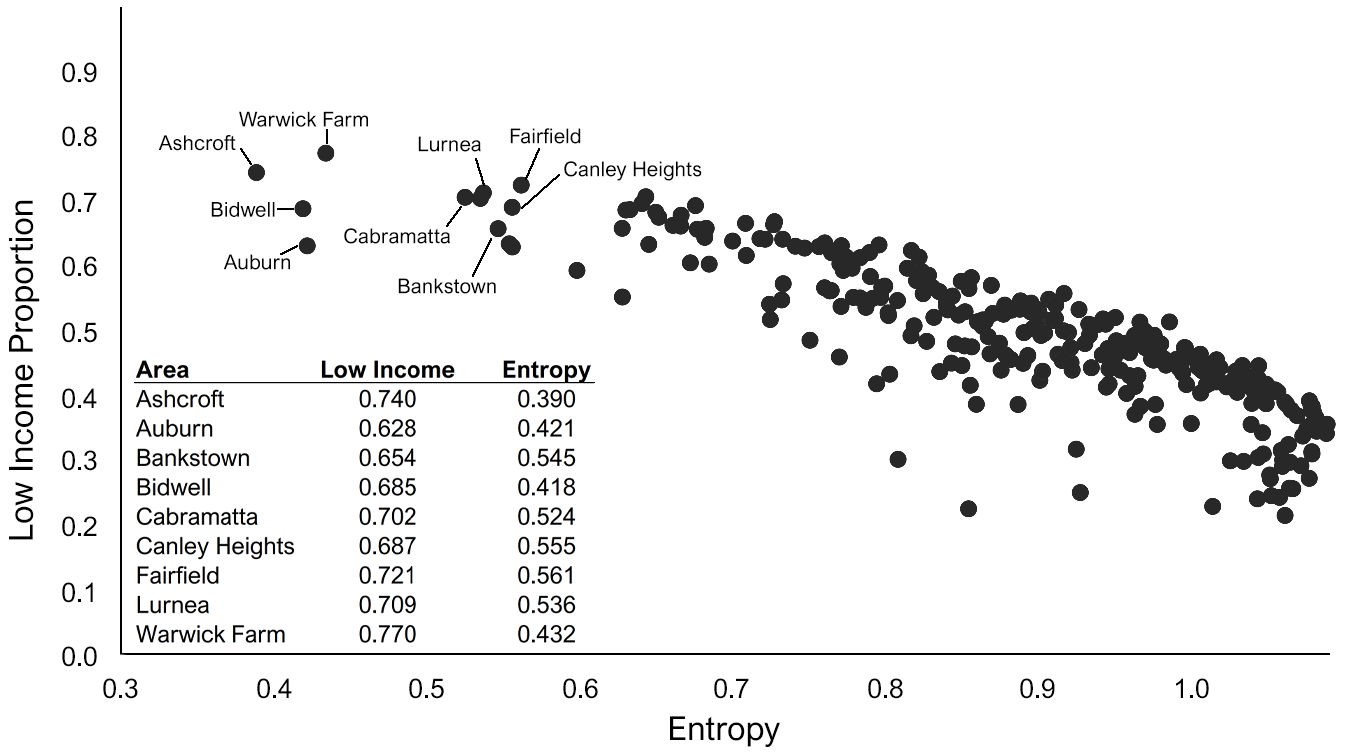
\includegraphics[width=0.85\textwidth]{body/figures/low-inc_ent.png}
    \caption{Caption}
    \label{fig:low_inc_ent}
\end{figure}

\begin{figure}[p]
    \centering
    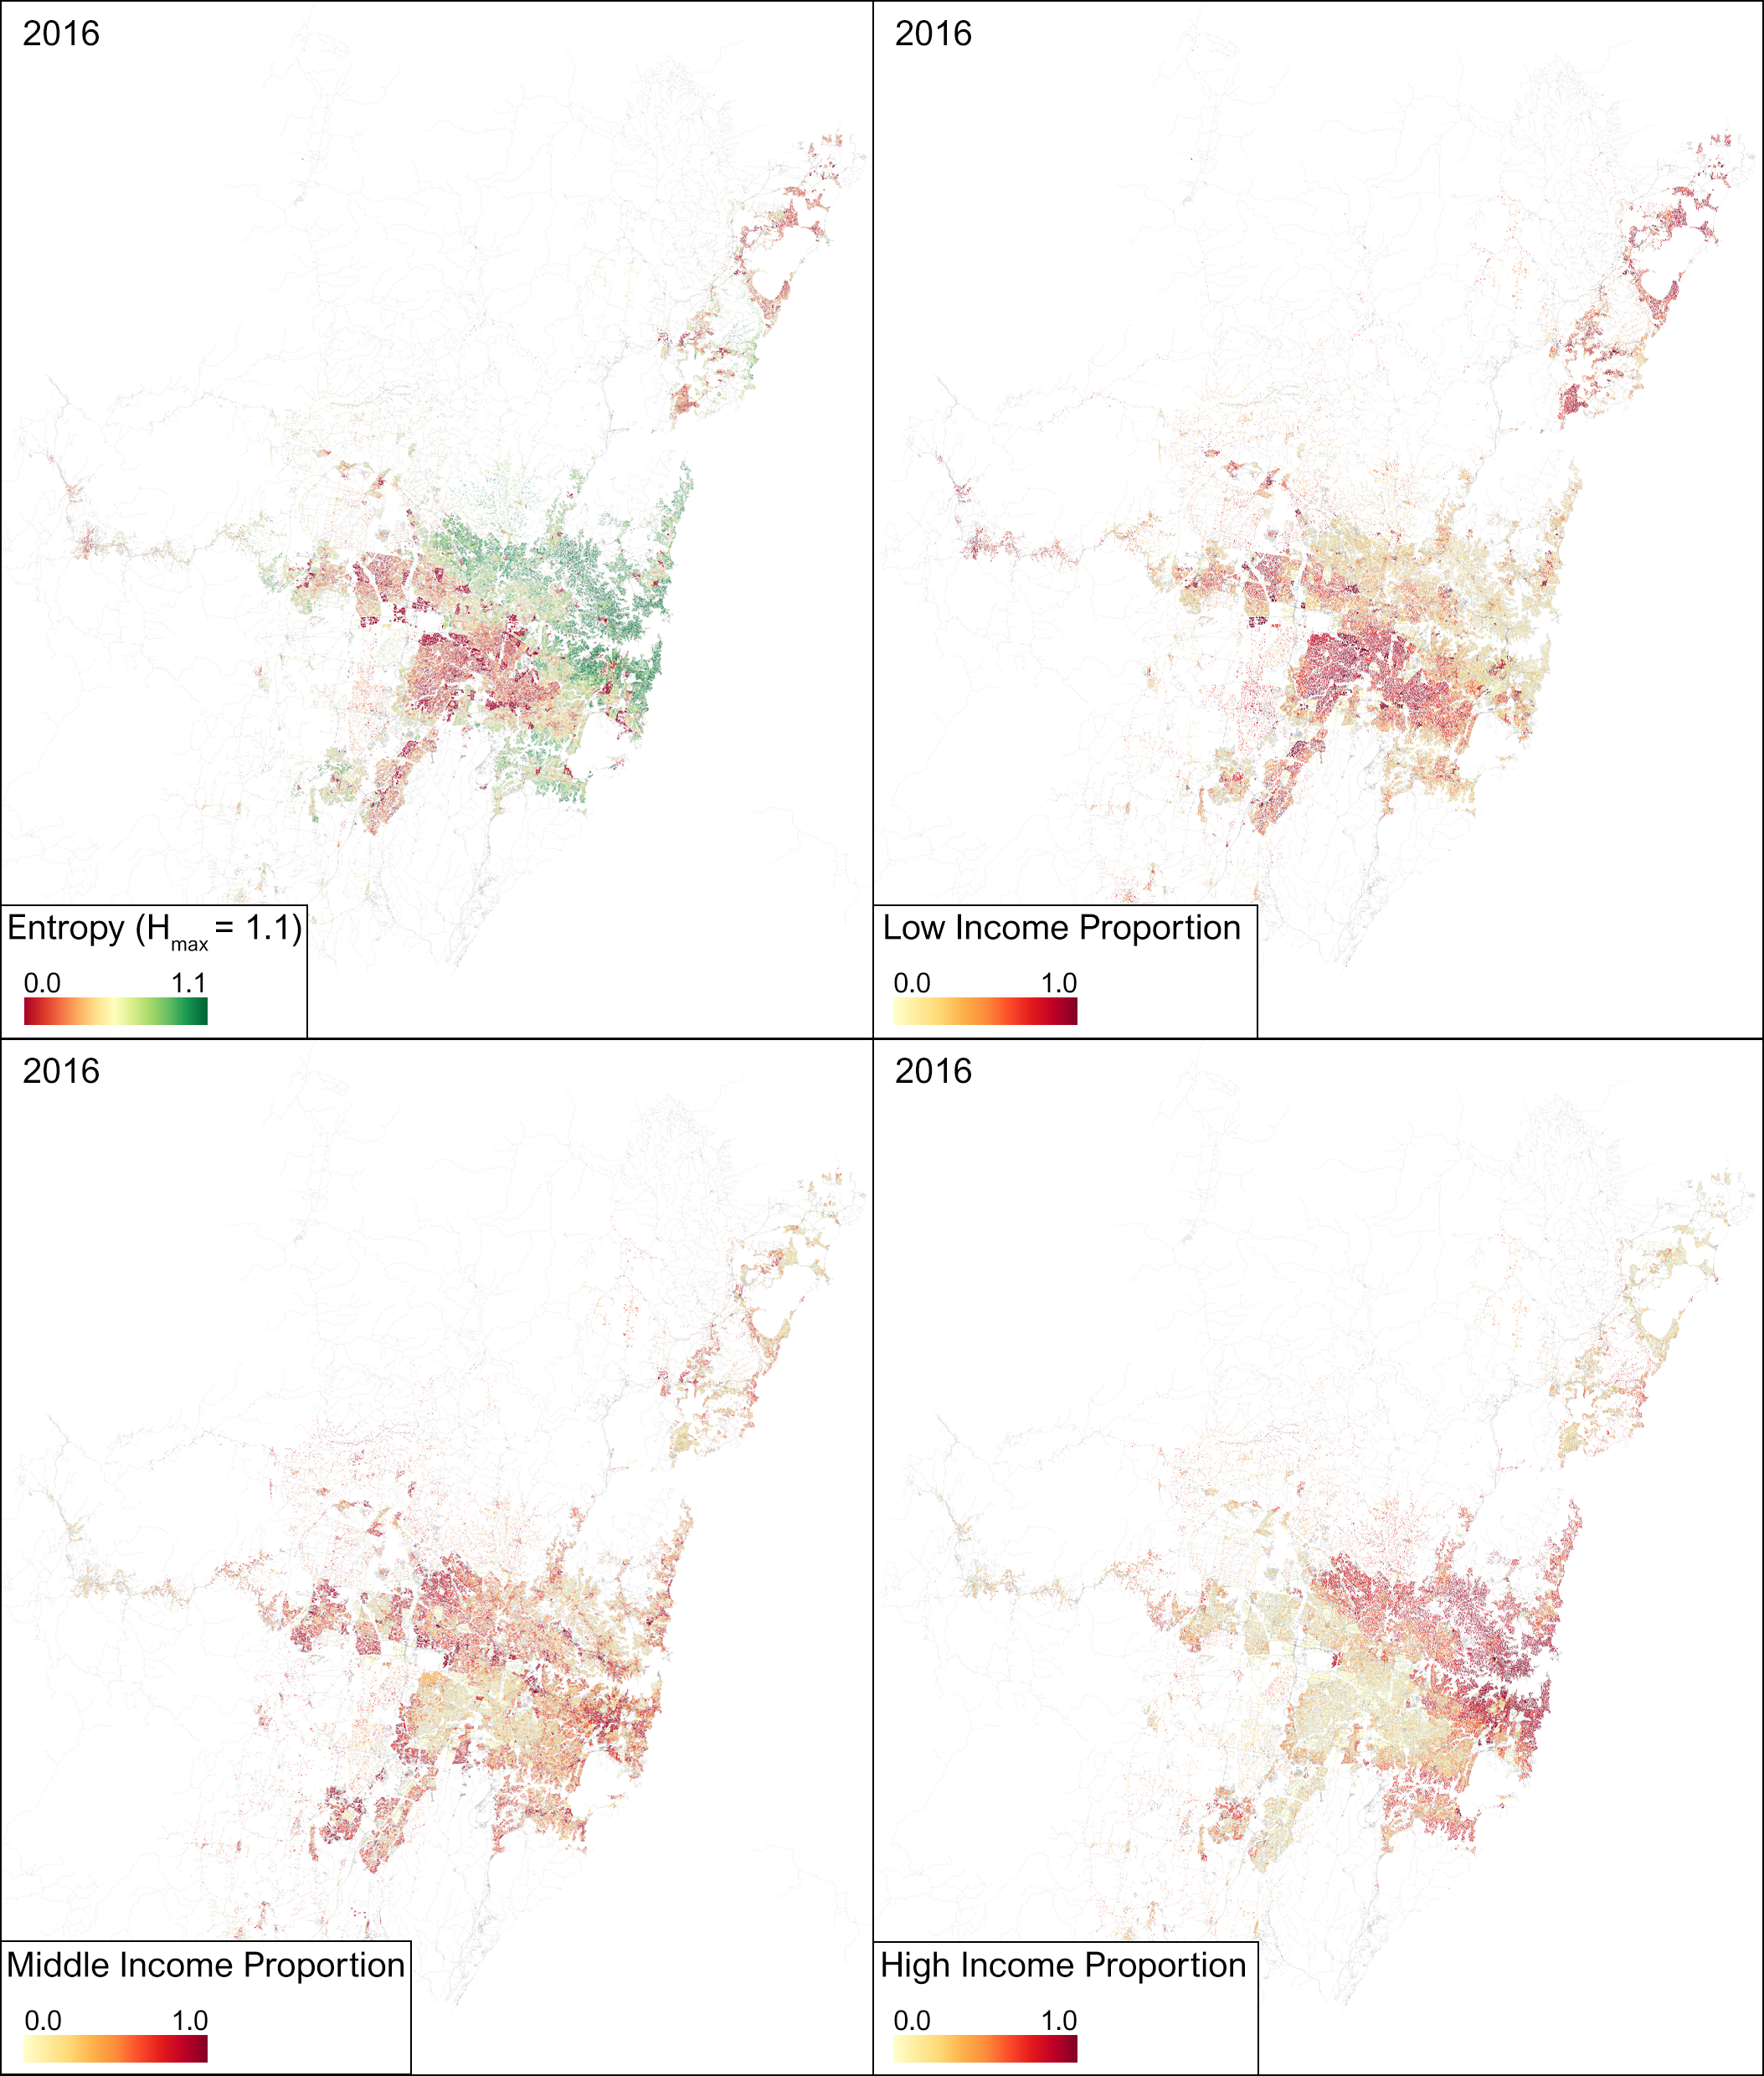
\includegraphics[width=1\textwidth]{body/figures/Income_Proportion_16.png}
    \caption{Caption}
    \label{fig:entropy_income}
\end{figure}

No doubt, this cursory evaluation does hint towards a possible degree of socioeconomic segregation in GS; however, a disaggregated view of income distributions is needed to investigate whether the prominence of low-income groups is a consistent mainstay of areas of low-diversity. Figure \ref{fig:entropy_income} illustrates the spatial distribution of entropy and all incomes groups in view of this. It is evident from this visualisation that the spread of entropy values show a relatively clear delineation between low-- and high-- diversity areas in GS, with lower entropy areas concentrated in the Central and Western suburbs of GS. Included in these areas are the suburbs within Fairfield, Merrylands, Auburn, and Mount Druitt. In these areas, the diversity index is estimated to range between 0.00 to ; which, coincidentally, also have the highest proportions of low-income earners in GS (ref. Figure \ref{fig:low_inc_ent}). Here, low-income groups constitute between 63 to 77 per cent of the population --- often, with less than 2 per cent belonging to high-income groups (ref. Figure \ref{fig:low_inc_ent}).\\

\textbf{** what is the history of these areas? ** why do they have so much more poorer people? ** is it a function of real estate? or public housing?}\\

\begin{figure}[!ht]
    \centering
    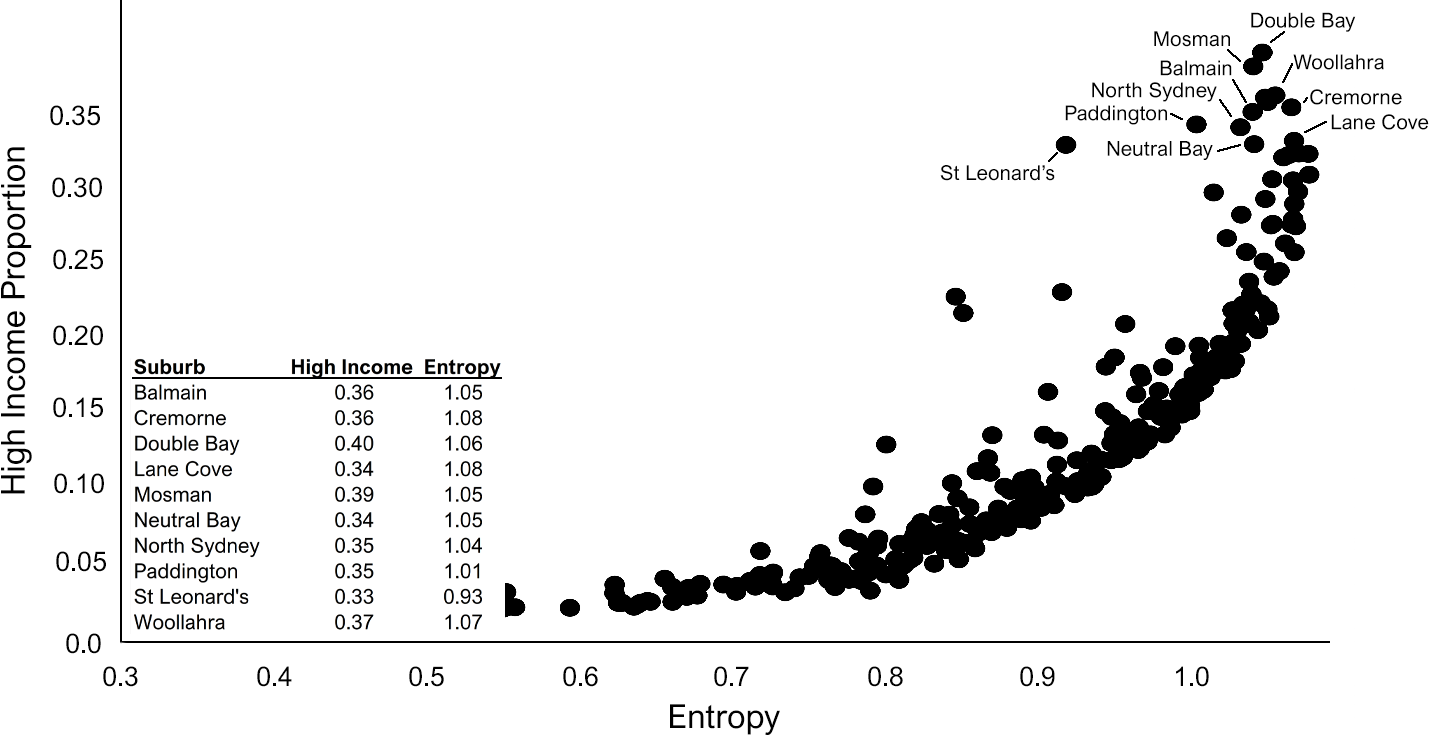
\includegraphics[width=0.85\textwidth]{body/figures/high-inc_ent.png}
    \caption{Caption}
    \label{fig:high-inc_ent}
\end{figure}


When considered in line with the distribution of high-income groups, it is worth pondering on the reason these areas do not exhibit similar segregation seen with low-income areas. From the results displayed in Table \ref{tab:entropy_incomes}, the distribution high-income groups have already shown to be negatively correlated with the lowest earners ($R=-0.57$) in Sydney, which alludes to the spatial division between both groups. However, it is interesting to note that, despite this disparity, high-income groups also occupy those areas with the highest entropy values. These are areas that tend to more proximate to the Sydney City Centre, with the highest $H$ values found in the suburbs around Mosman, North Sydney, the Eastern Suburbs, and Manley. In these suburbs, approximately 33 per cent to 40 per cent of the population within these areas fall within the high-income bracket (ref. Figure \ref{fig:high-inc_ent}). The results suggest that their relative diversity is due to the spatial overlaps seen with middle-income earners ($R=0.57$), who also tend to occupy these same areas.\\

\textbf{** what do these areas have in common? ** why are there no areas where there is high-income only? ** is there planning policy that prevents this?}\\


\subsection{Accessibility and Incomes}

\begin{figure}[!ht]
    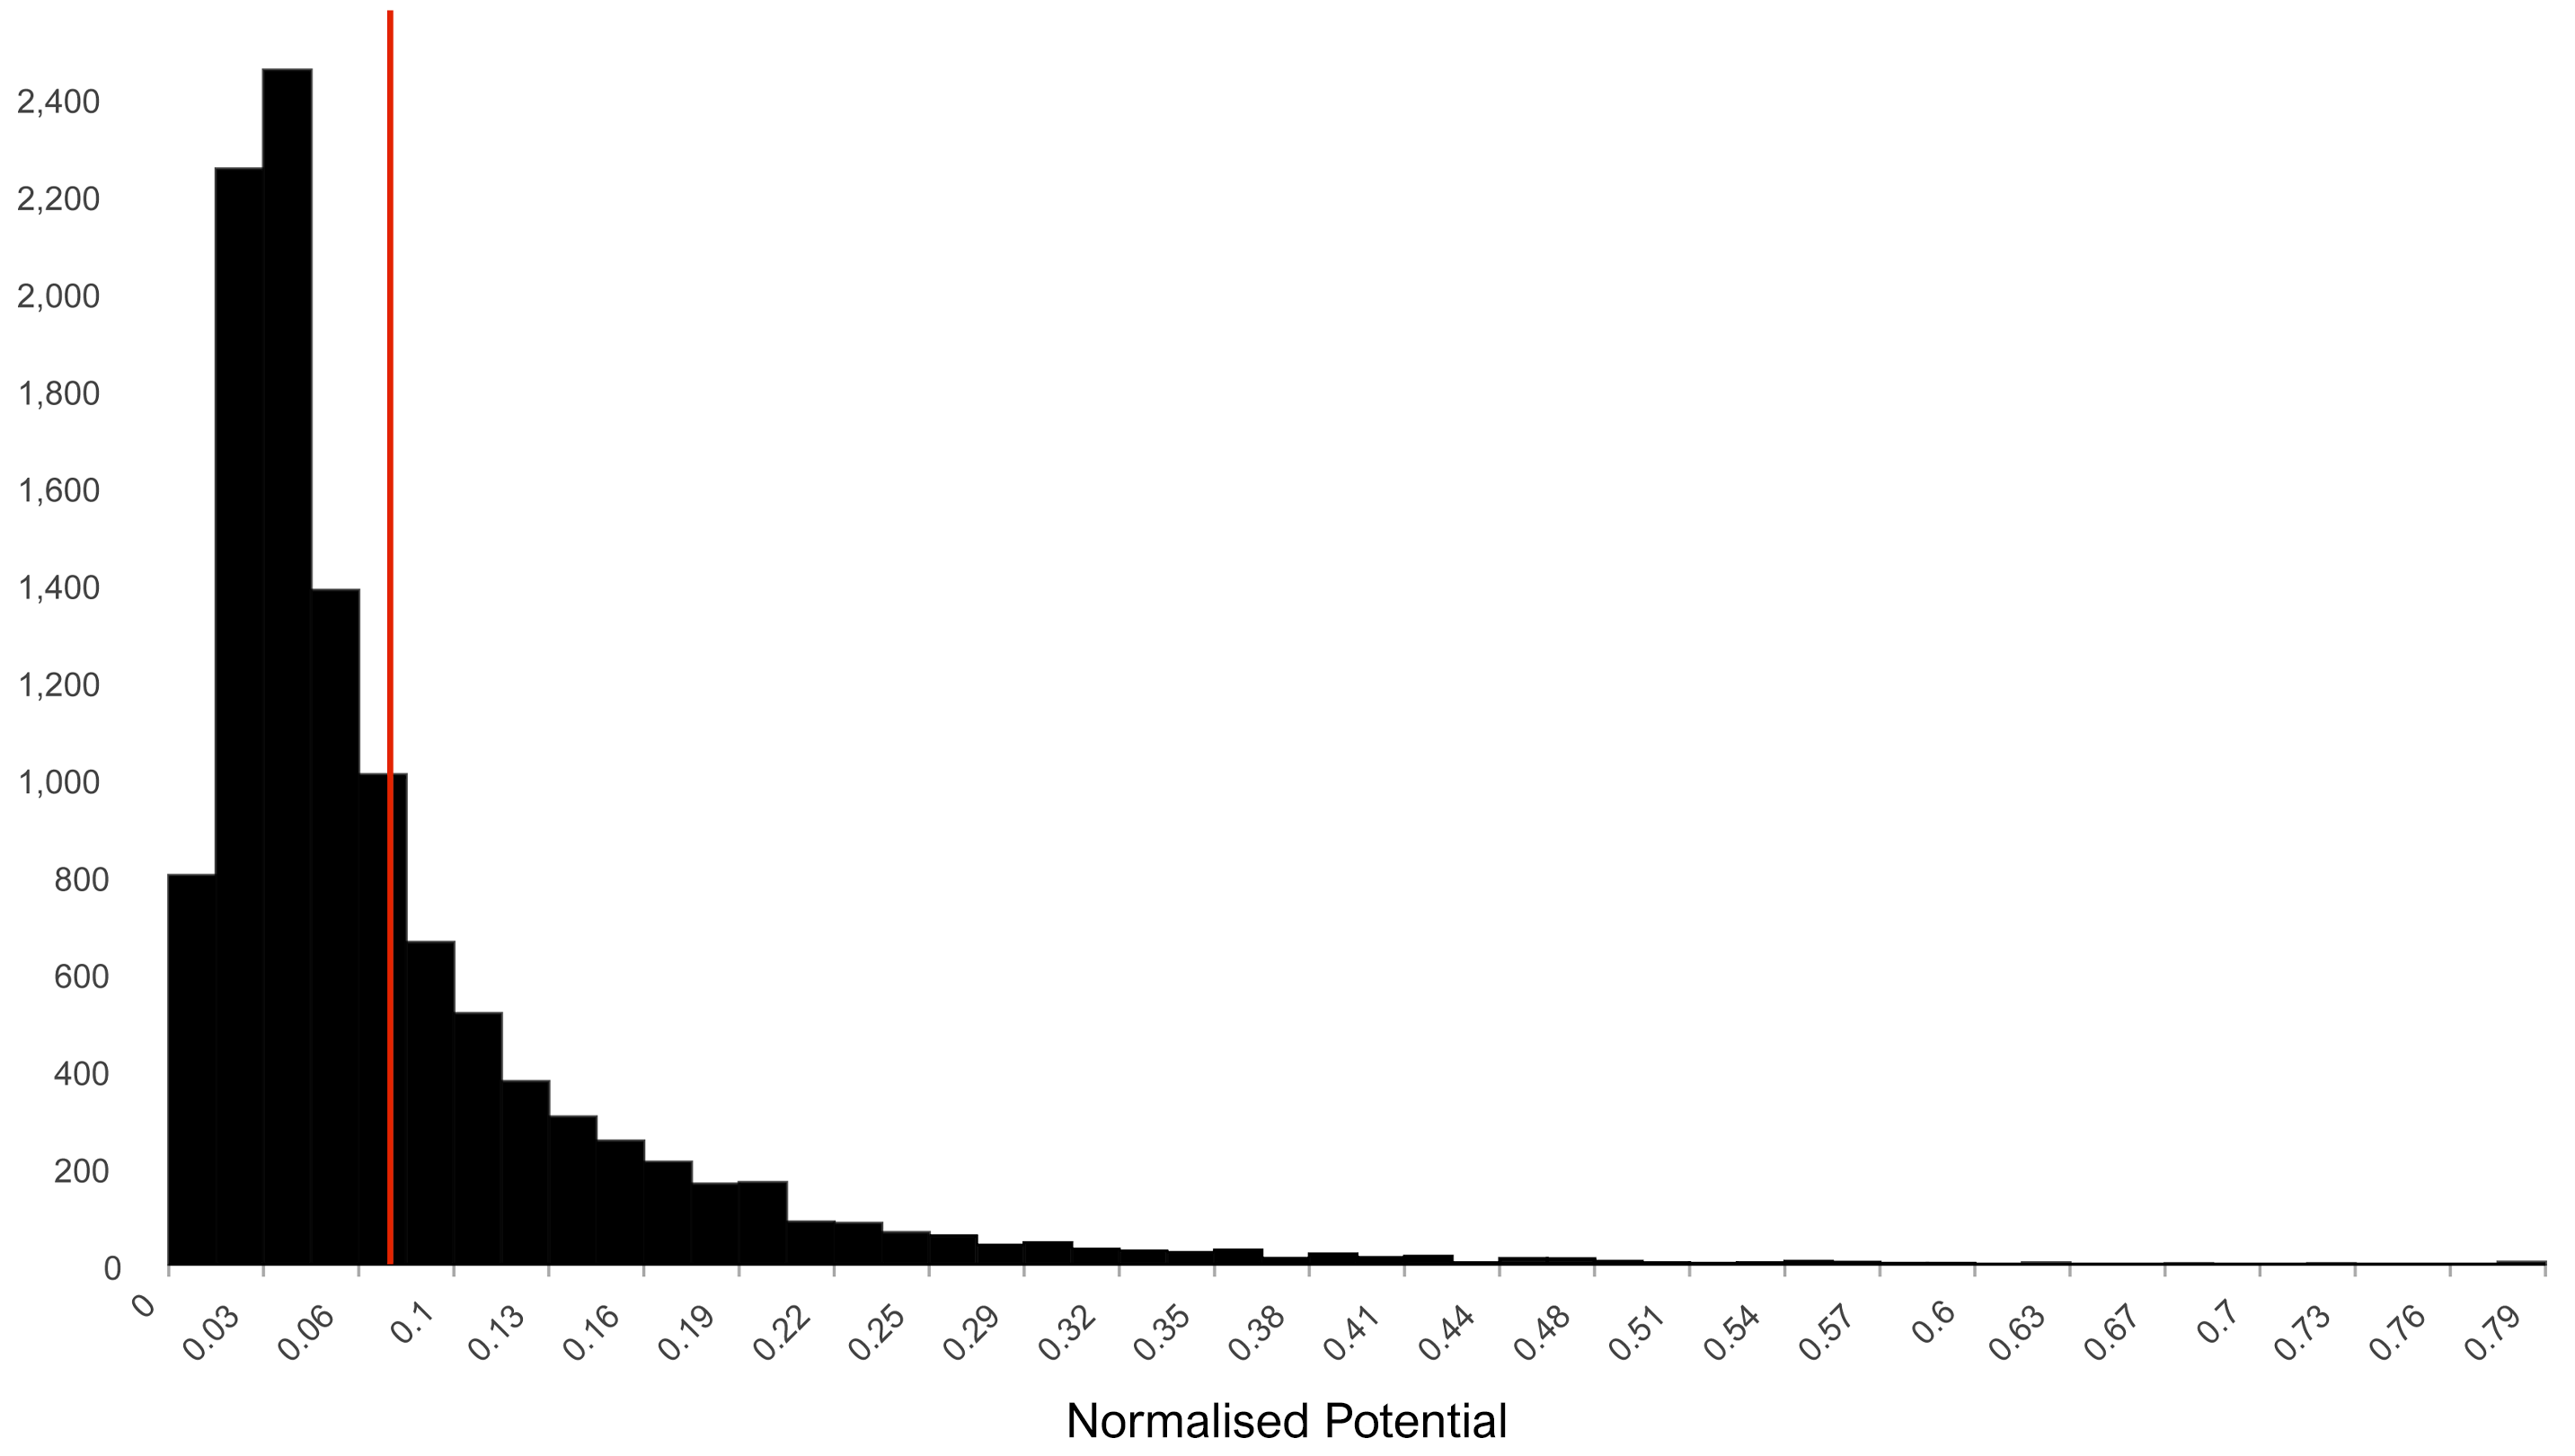
\includegraphics[width=0.9\textwidth]{body/figures/accessibility_histogram.png}
    \caption{Bivariate Graphs: 2016 Accessibility and Income Segregation}
    \label{fig:access_hist}
\end{figure}

The results above have now quantified the spatial delineation between income groups in Sydney. It has illustrated the possible sociospatial isolation that lower income groups may be affronted with given their distribution within GS. As such, it raises the concerns as to whether these income groups may disproportionately experience the same negative spatial externalities seen in many cities globally. This paper thus seeks to now investigate whether any variances in accessibility are observed in line with  GS's observed income spread. The distribution of accessibility scores, computed from the gravity potential model, are displayed in Figure \ref{fig:access_hist}. The normalised potential accessibility score was estimated to range between 0.01 to 0.78, with a mean score of 0.07. The highest potential scores were noted in those suburbs within-- and proximate to-- Sydney's Inner City, North Sydney, Mascot, Carlingford, Chatswood, and Parramatta. These areas hold the highest employment densities concentrating approximately 40 per cent of all within the GS area. Model estimates indicate that the Sydney Inner City area constitute approximately 22.5 per cent of all metropolitan employment movement. This is a figure also reflected in the JTW census data, in which the area recorded a 22.7 per cent share of Sydney's total working population in 2016. \\

\begin{figure}[!ht]
    \centering
    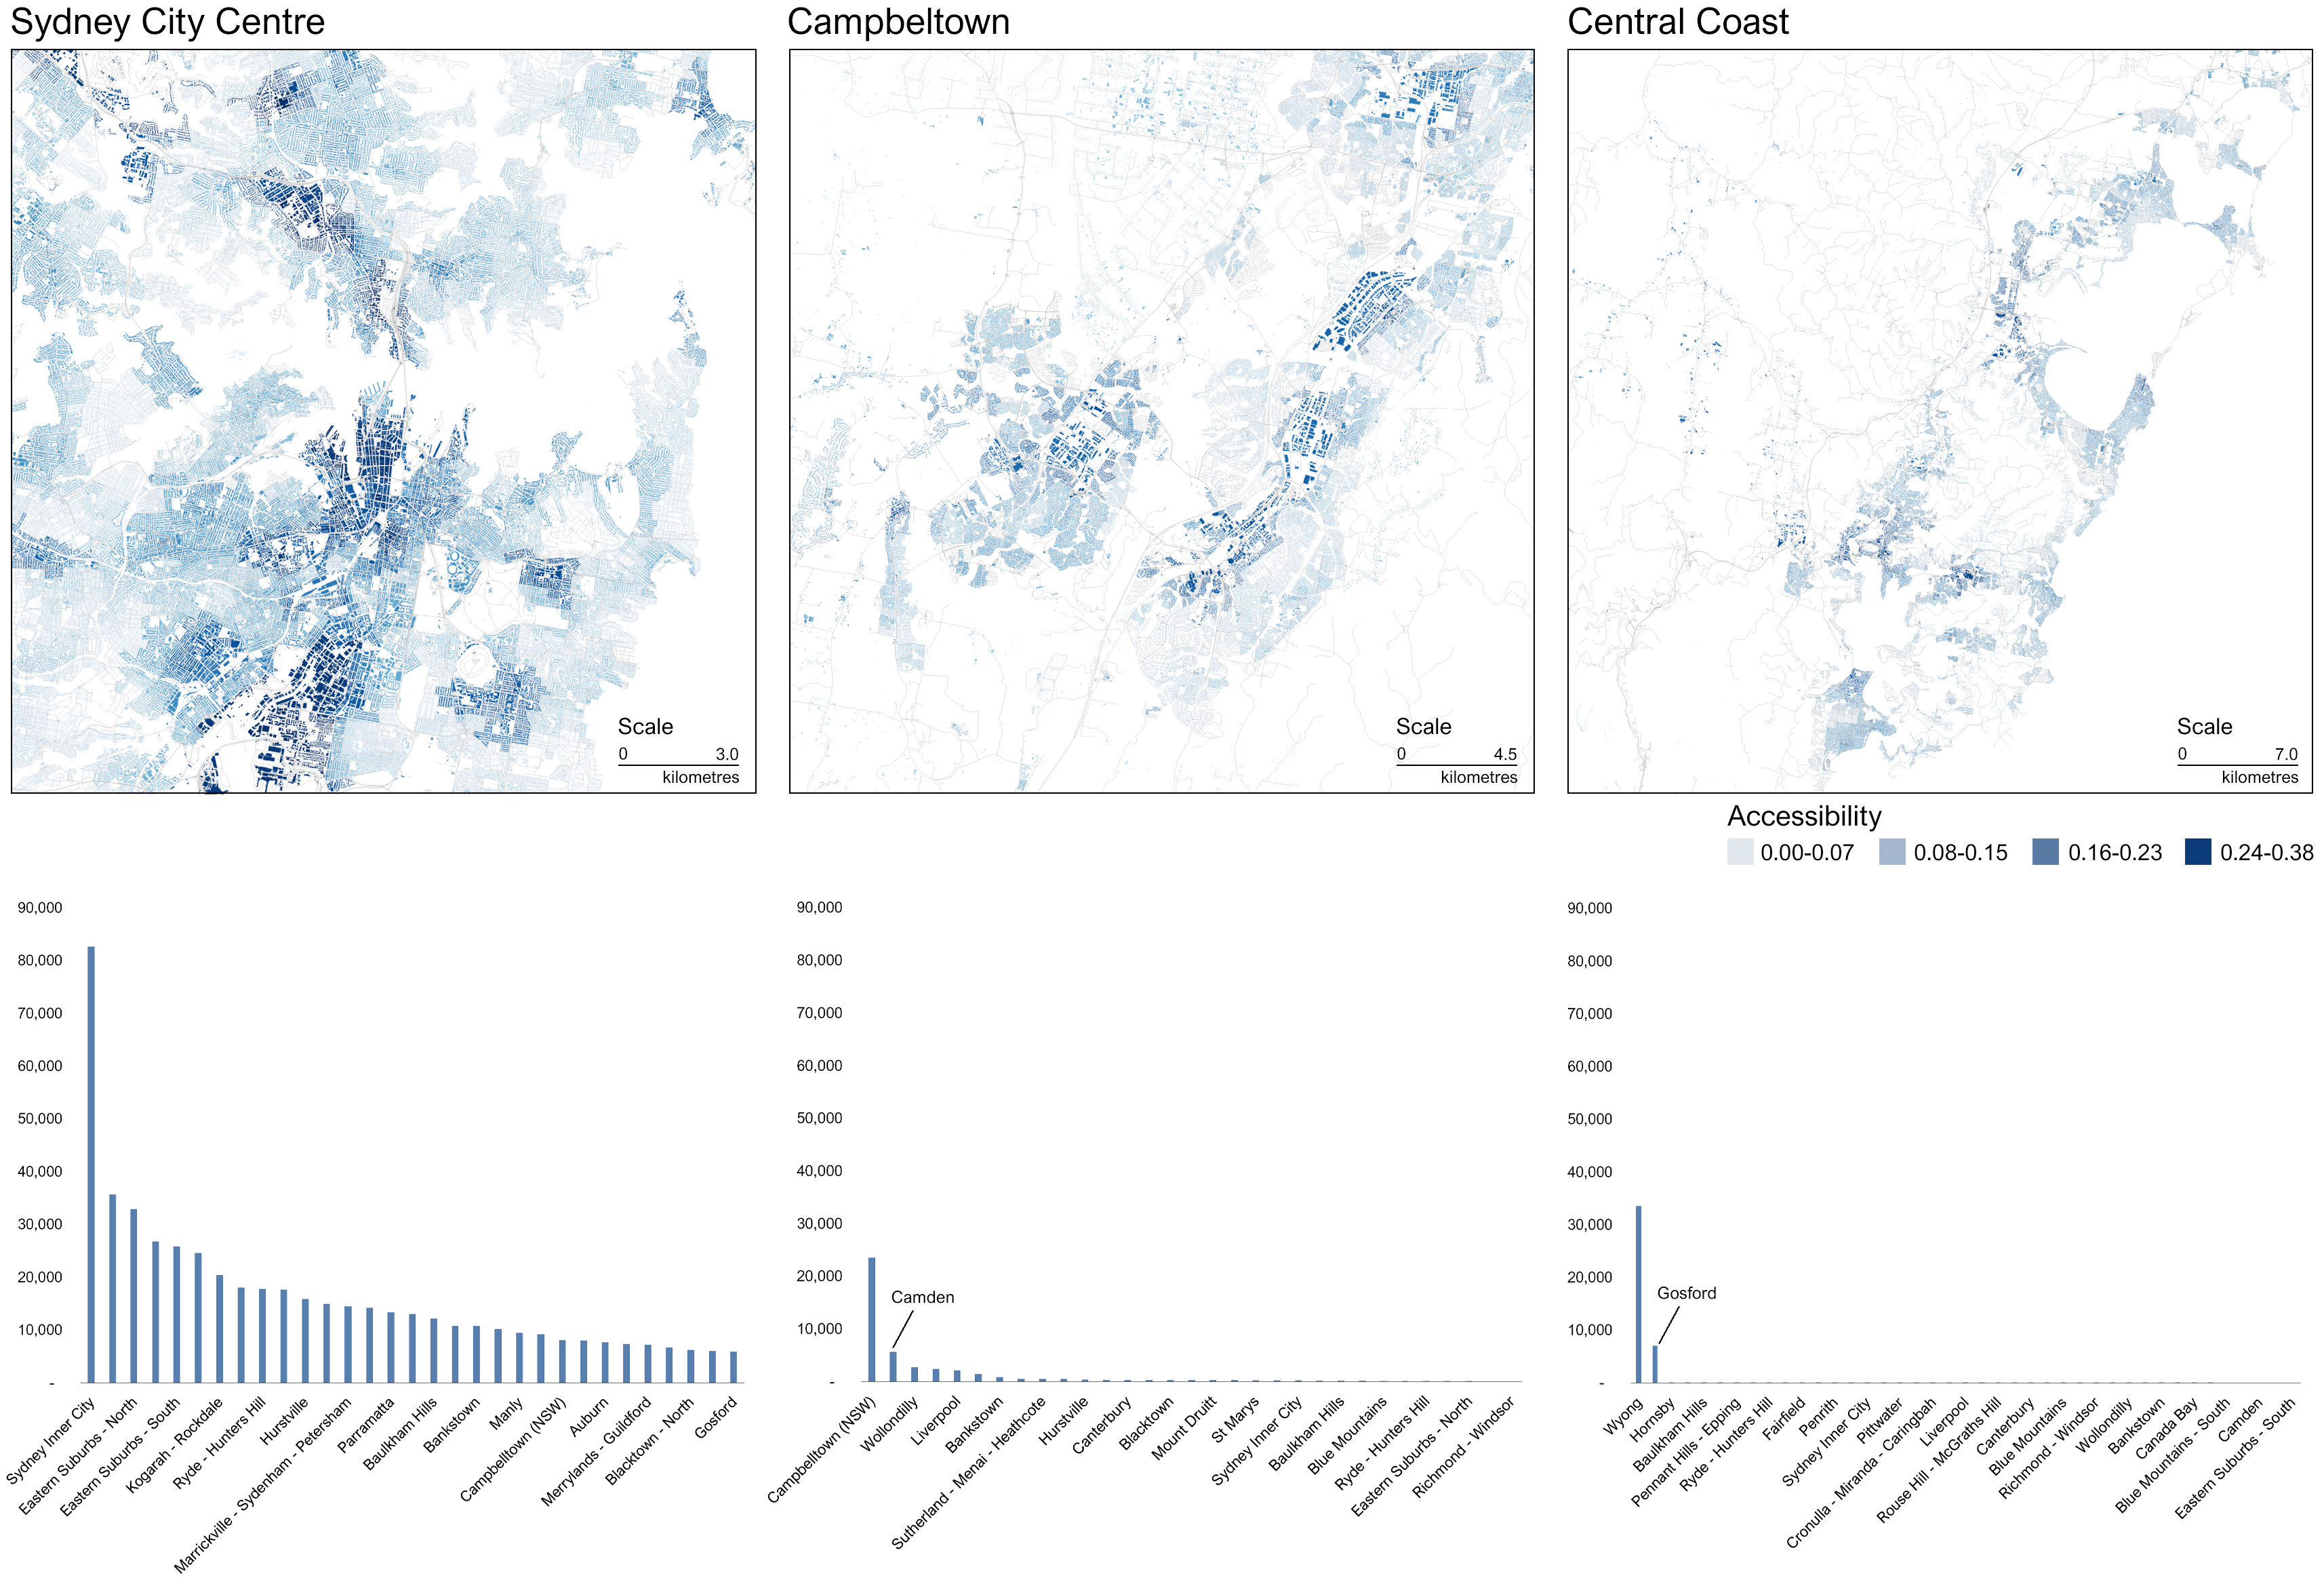
\includegraphics[width=1\textwidth]{body/figures/access_flows.png}
    \caption{Caption}
    \label{fig:access-flows}
\end{figure}

Conversely, it is interesting to note that the spatial distribution of lower potential accessibility scores appears relatively more evenly throughout many suburbs across the GS metropolitan.  The median potential score of these areas is estimated to be approximately 0.04. This potential score comes despite a relatively substantial number of smaller employment loci available (e.g., Ashfield, Burwood, Balgowlah, Clemton Park, Kogarah, Marrickville) within these largely suburban areas. The findings suggest that, despite these smaller pockets of employment, the Sydney City Centre, North Sydney, Parramatta, and Chatswood remain the most significant employment clusters within the GS system. Several exceptions to this are noted within the GS periphery however. In more distal areas, such as Katoomba, Campbelltown, and Gosford, potential accessibility scores remain relatively high. This deviation is likely attributed to large intervening distances between these areas to Sydney's primary employment hubs. As a result, these areas appear to have a secondary role in centralising employment flows within Sydney, particularly at the metropolitan's periphery. This centralising pattern of movement is also captured within the accessibility model's estimated flows. For example, between Sydney City and Campbelltown, there is a clear distinction between the source of movement within both these locations (ref. Figure \ref{fig:access-flows}). Where Sydney City sees movement from all suburbs across GS; within Campbeltown, model estimates indicate predominantly inter-zonal movement, with more modest population flows from Camden, Liverpool, and Bankstown. In contrast to these flows, peripheral zones, such as the Central Coast, form a separate employment locus given this distance. Resultingly, accessibility remains relatively high given that employment flows are seen to be almost exclusively circumscribed to within the region (ref. Figure \ref{fig:access-flows}). \\

\textbf{Sense check needed: are these flows correct? Is there negligible movement from Sydney City to central coast for work?}


\begin{sidewaysfigure}[p]
    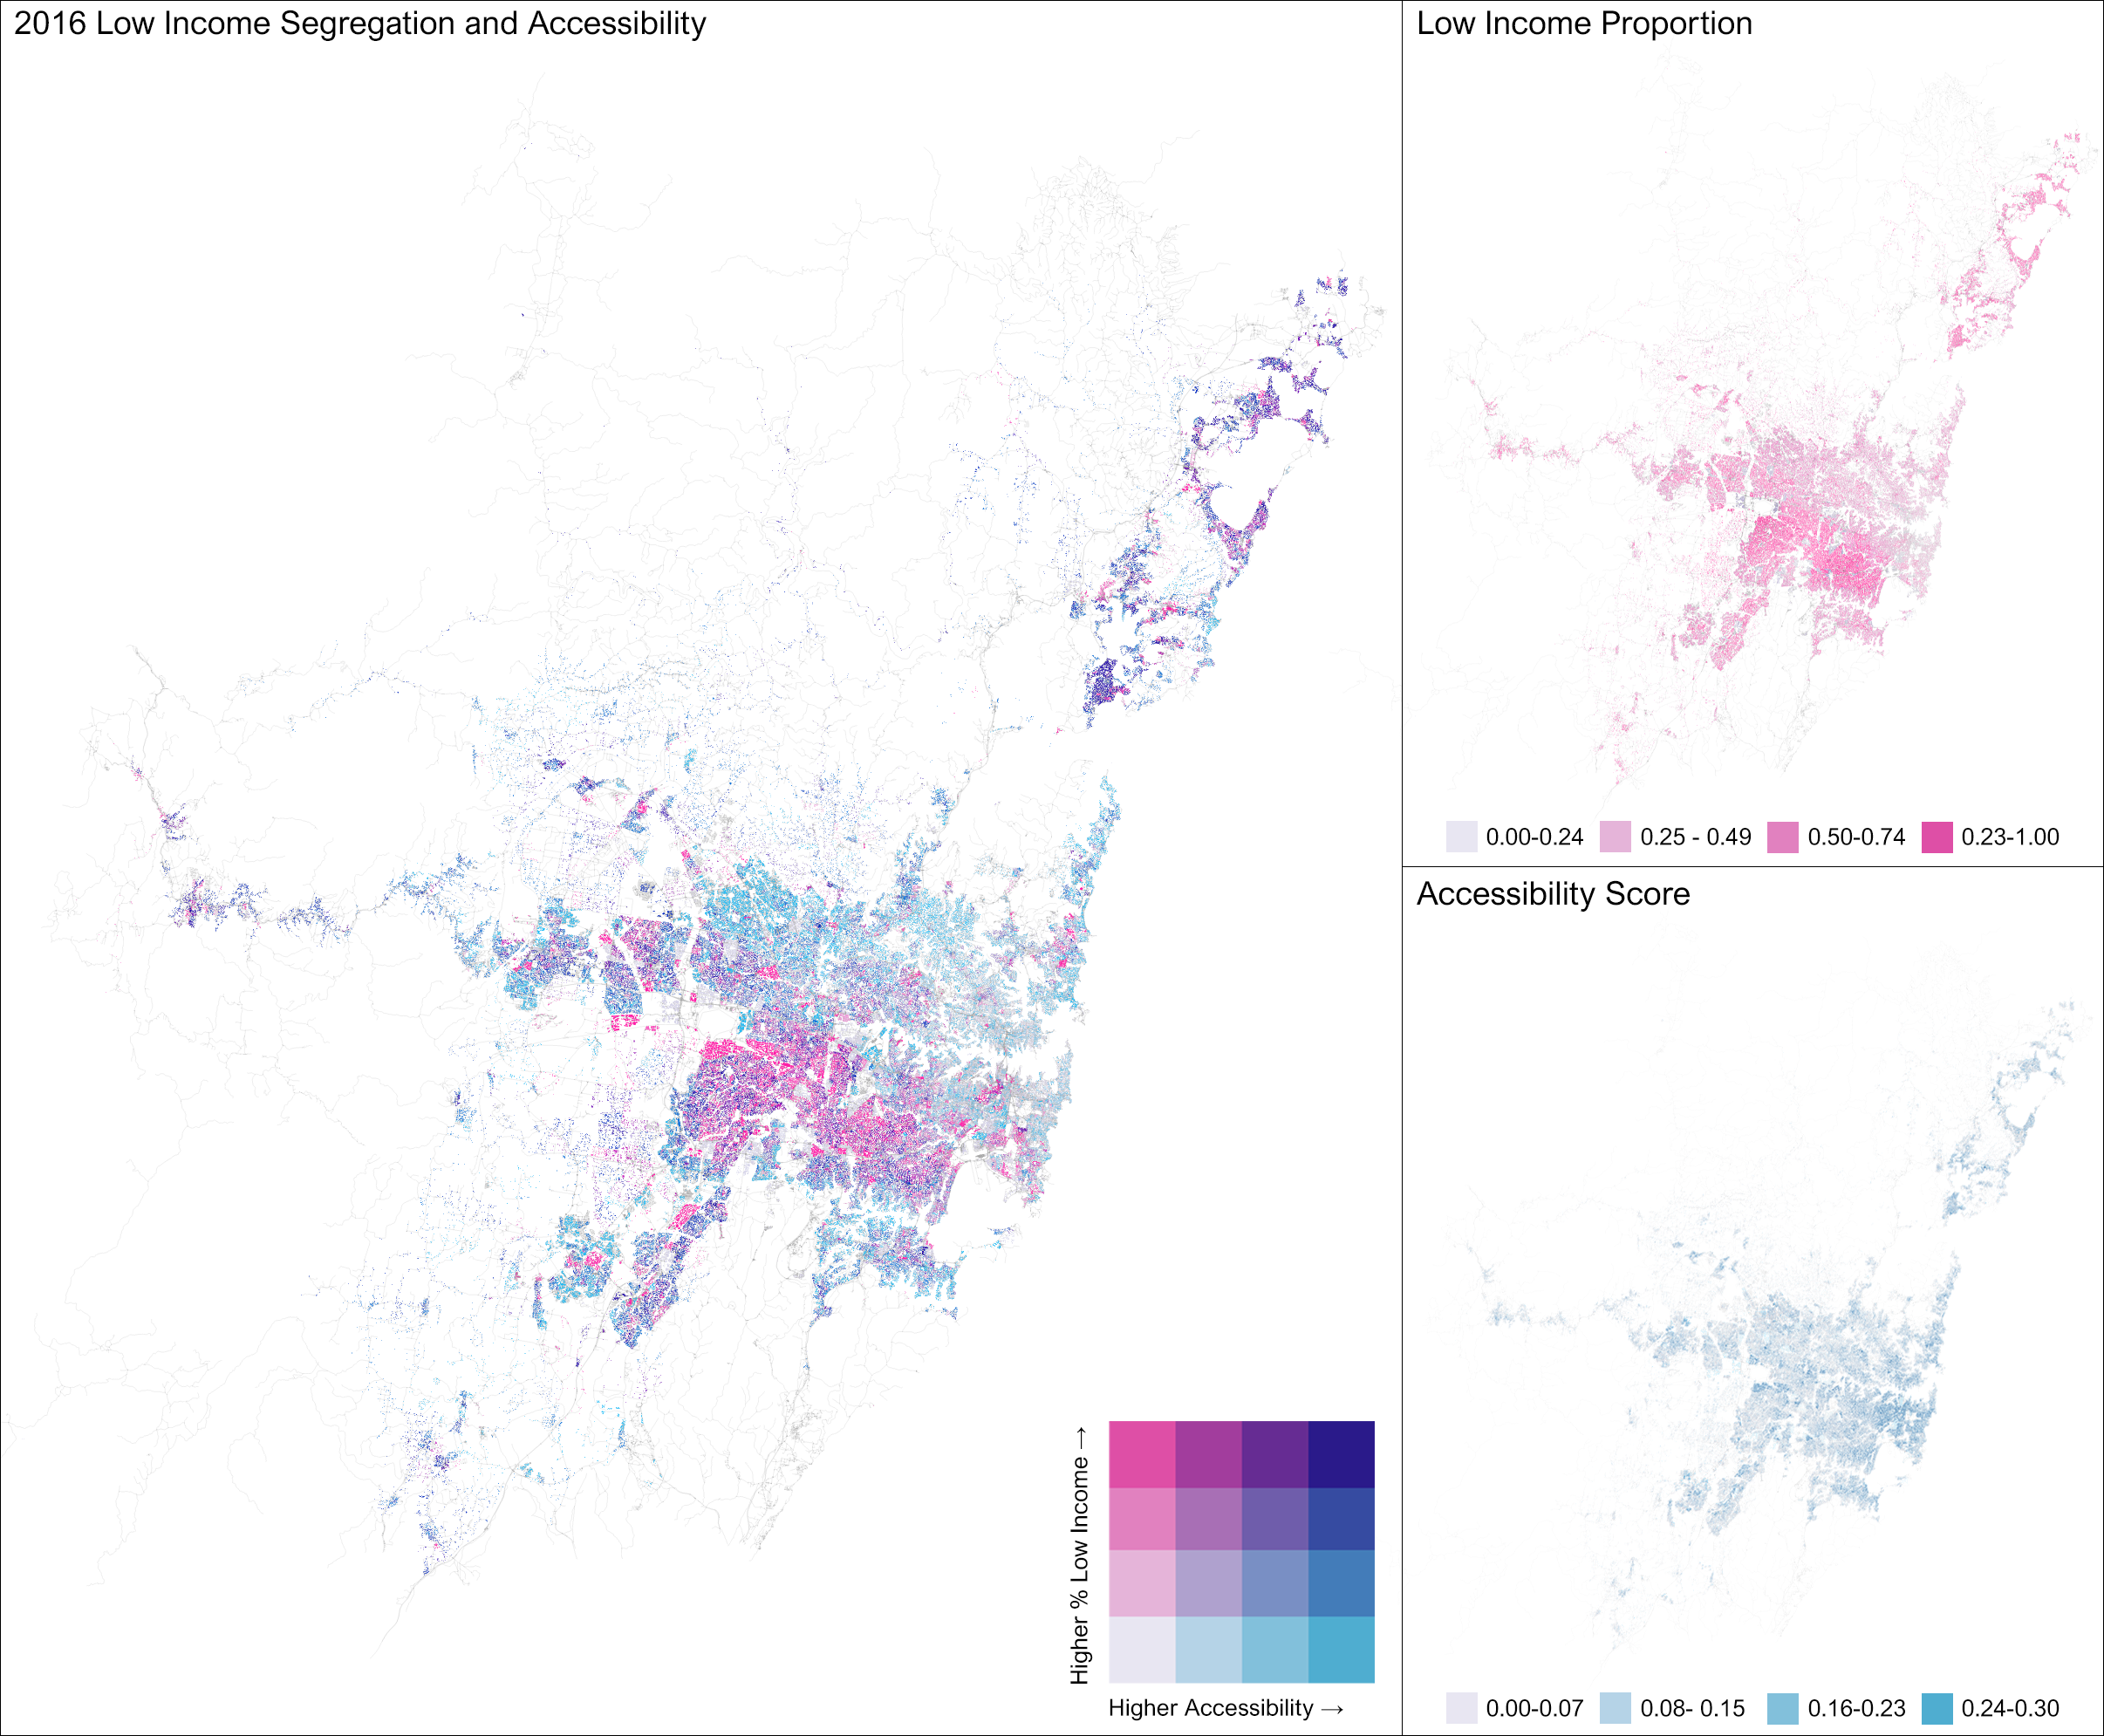
\includegraphics[width=1\textwidth]{body/figures/low_inc_16.png}
    \caption{Bivariate Graphs: 2016 Accessibility and Income Segregation}
    \label{fig:access_income}
\end{sidewaysfigure}

Considering these flow trends in line with the spatial variances in accessibility, attention should be drawn to those intermediary zones that fall in between Sydney's' major employment hub where low accessibility is noted throughout. These areas are typified by low-density, residential land-uses. The greater topological distances to GS's employment centres draws attention to the disparate costs that may be experienced by resident populations; thus, it reiterates the need to better understand these accessibility costs in view of their socioeconomic structures.  Figure \ref{fig:access_income} illustrates the distribution of accessibility scores relative to that of low-income groups. It is interesting to note that, whilst low-income groups can generally be delineated within Sydney's inner Southwest--, Southwest--, and Blacktown-- suburbs, there does not appear to be any clear correlation in accessibility variances within these areas ($R^2=0.01$). Resultingly, the findings cannot support previous assumptions of socioeconomic stratification and isolation. \\

In this sense, employment accessibility appears to be experienced equally across income groups within Sydney. However, at this juncture, it is worth repeating that employment density is taken as a proxy to area attractiveness. Certainly, whilst this does look to be a relatively useful measure of Sydney's employment movement, no measure of employment type-- or quality-- has been taken into account within the current accessibility model. It is also worth repeating that accessibility in Sydney has been shown to be pervasively low throughout the metropolitan, with the exception of those areas adjacent to Sydney City, Chatswood, and Parramatta. As such, whilst no spatial disadvantages can be attributed to lower-income areas in this study, further work is required to ascertain whether these disadvantages are seen perhaps in the quality and type of employment. This proposes the idea the available employment centres may not necessarily meet the demands of their resident and immediate populations. As such, the presence of a proximate employment centre does not contribute to improving or equally distributing economic opportunities. \\

\textbf{Nevertheless, the results do not display an significant relationship between employment accessibility and the income-groups}.

\subsection{The Influence of Accessibility and Incomes on House Prices in Sydney}

Having now considered the relationship between income groups and accessibility, this paper now shifts towards understanding if these variables may also be alternatively reflected in house prices. First, an OLS regression was conducted to understand the house prices may be affected by these variables within the entire system. The results of the test is indicated in Table \ref{tab:ols_results}. The model performance indicates a multiple-- and adjusted-- $R^2$ value of 0.81 for both, which indicates a fairly strong linear relationship across all variables whereby over 80 per cent of the model variances (normalised through a logarithmic transformation) can be accounted for by the independent variables. For the most part, the results of the OLS model indicate a fairly predictable relationship between house prices and the independent variables used. House prices are noted to markedly increase with size (as proxied by the number of bedrooms, bathrooms, and parking spaces, as well as increasing distances from major infrastructure features and major recreational sport facilities. This comes in addition to the negligible increases in house prices are also seen with increasing distances from educational facilities, and shopping centres. As also expected, negative changes in house prices are also linked to as distance from Sydney City, coastlines, and reduced crime rates. \\

\renewcommand{\baselinestretch}{0.8}
\begin{table}[!ht]
  \centering \small
    \begin{tabular}{lccccc}
    \textbf{Residuals:} &       &       &       &       &  \\
    \midrule
          & \multicolumn{1}{c}{\textbf{Min}} & \multicolumn{1}{c}{\textbf{1Q}} & \multicolumn{1}{c}{\textbf{Median}} & \multicolumn{1}{c}{\textbf{3Q}} & \multicolumn{1}{c}{\textbf{Max}} \\
          & -3.08558 & -0.14556 & -0.01844 & 0.11633 & 2.40827 \\
          &       &       &       &       &  \\
    \textbf{Coefficients:} &       &       &       &       &  \\
    \midrule
          & \multicolumn{1}{c}{\textbf{Estimate}} & \multicolumn{1}{c}{\textbf{Std. Error}} & \multicolumn{1}{c}{\textbf{t-value}} & \multicolumn{1}{c}{\textbf{Pr($>$ $|$ t $|$ )}} &  \\
    (Intercept) & 1.33E+01 & 5.69E-02 & 233.182 & \multicolumn{1}{c}{$<$2.00E-6} & \multicolumn{1}{l}{***} \\
    Bedrooms & 1.42E-01 & 1.58E-03 & 90.152 & \multicolumn{1}{c}{$<$2.00E-6} & \multicolumn{1}{l}{***} \\
    Bathrooms & 4.89E-02 & 1.48E-03 & 33.016 & \multicolumn{1}{c}{$<$2.00E-6} & \multicolumn{1}{l}{***} \\
    Distance to Sydney & -1.45E-05 & 1.69E-07 & -85.66 & \multicolumn{1}{c}{$<$2.00E-6} & \multicolumn{1}{l}{***} \\
    Distance to Secondary City & 7.07E-07 & 1.74E-07 & 4.065 & 4.82E-05 & \multicolumn{1}{l}{***} \\
    Distance to Beach & -2.44E-06 & 2.24E-07 & -10.916 & \multicolumn{1}{c}{$<$2.00E-6} & \multicolumn{1}{l}{***} \\
    Distance to Bus Interchanges & 2.91E-06 & 4.83E-07 & 6.031 & 1.65E-09 & \multicolumn{1}{l}{***} \\
    Distance to Highway & 7.50E-06 & 4.44E-07 & 16.883 & \multicolumn{1}{c}{$<$2.00E-6} & \multicolumn{1}{l}{***} \\
    Distance to Primary School & 1.02E-05 & 3.26E-06 & 3.118 & 0.00182 & \multicolumn{1}{l}{**} \\
    Distance to University & 1.12E-06 & 4.27E-07 & 2.617 & 0.00889 & \multicolumn{1}{l}{**} \\
    Distance to Swimming Pool & -4.61E-06 & 9.32E-07 & -4.952 & 7.40E-07 & \multicolumn{1}{l}{***} \\
    Distance to Shopping Centre & 1.11E-05 & 7.50E-07 & 14.774 & \multicolumn{1}{c}{$<$2.00E-6} & \multicolumn{1}{l}{***} \\
    Distance to Sport Centre & 9.00E-06 & 7.27E-07 & 12.378 & \multicolumn{1}{c}{$<$2.00E-6} & \multicolumn{1}{l}{***} \\
    Population Above 65 & 5.08E-03 & 2.17E-04 & 23.355 & \multicolumn{1}{c}{$<$2.00E-6} & \multicolumn{1}{l}{***} \\
    Crime Rate & -4.35E-02 & 1.62E-02 & -2.681 & 0.00735 & \multicolumn{1}{l}{**} \\
    Low Income (\%) & -1.87E-01 & 5.75E-02 & -3.244 & 0.00118 & \multicolumn{1}{l}{**} \\
    Middle Income (\%) & -1.02E-01 & 5.80E-02 & -1.758 & 0.0788 & \multicolumn{1}{l}{.} \\
    High Income (\%) & 2.51E+00 & 5.97E-02 & 41.983 & \multicolumn{1}{c}{$<$2.00E-6} & \multicolumn{1}{l}{***} \\
    Accessibility Score & 2.73E-01 & 8.68E-02 & 3.142 & 0.00168 & \multicolumn{1}{l}{**} \\
    \midrule
    Significance Codes: &       &       &       &       &  \\
    \multicolumn{6}{c}{ 0 ‘***’ 0.001 ‘**’ 0.01 ‘*’ 0.05 ‘.’ 0.1 ‘ ’ 1} \\
    \textit{Number of data points: 32,050} &       &       &       &       &  \\
    \multicolumn{6}{l}{\textit{Residual standard error: 0.2455 on 32,049 degrees of freedom}} \\
    \multicolumn{6}{l}{\textit{Multiple R-squared: 0.8103, Adjusted R-squared: 0.8102}} \\
    \multicolumn{6}{l}{\textit{F-statistic: 7,604 on 18 and 32,049 DF,  p-value: $<$2.2e-16}} \\
    \multicolumn{6}{l}{\textit{Residual sum of squares: 1,931.751}} \\
    \multicolumn{6}{l}{\textit{AIC:  952.1797}} \\
    \multicolumn{6}{l}{\textit{AICc:  952.2059}}
    \end{tabular}%
    \caption{Add caption}
  \label{tab:ols_results}%
\end{table}%

However, in view of this study, it is interesting to note the differences in significance levels both income groups and accessibility scores display on house prices. The OLS model indicates that the presence of both low-- and high-- income groups are relatively sound predictors for the variance in house prices in GS, with the model indicating a significance level of at least 99 per cent. Accessibility scores also look be significant at the global level, with a $p-value$ of less than 0.01. As denoted within the model, increasing proportions of low-- and high-- income groups display a relative change of -0.2 and 2.5 per cent change in house price, respectively. Further, at the metropolitan level, relative rise of 0.3 per cent is with house prices within areas that have increased accessibility. It is worth noting that the presence of middle-income groups, as defined in this study, do not indicate the same level of predictive potential. This is likely due to their larger aggregation of income into a single group; and, resultingly, their relatively even distribution throughout all of GS. \\

\begin{figure}[!ht]
    \centering
    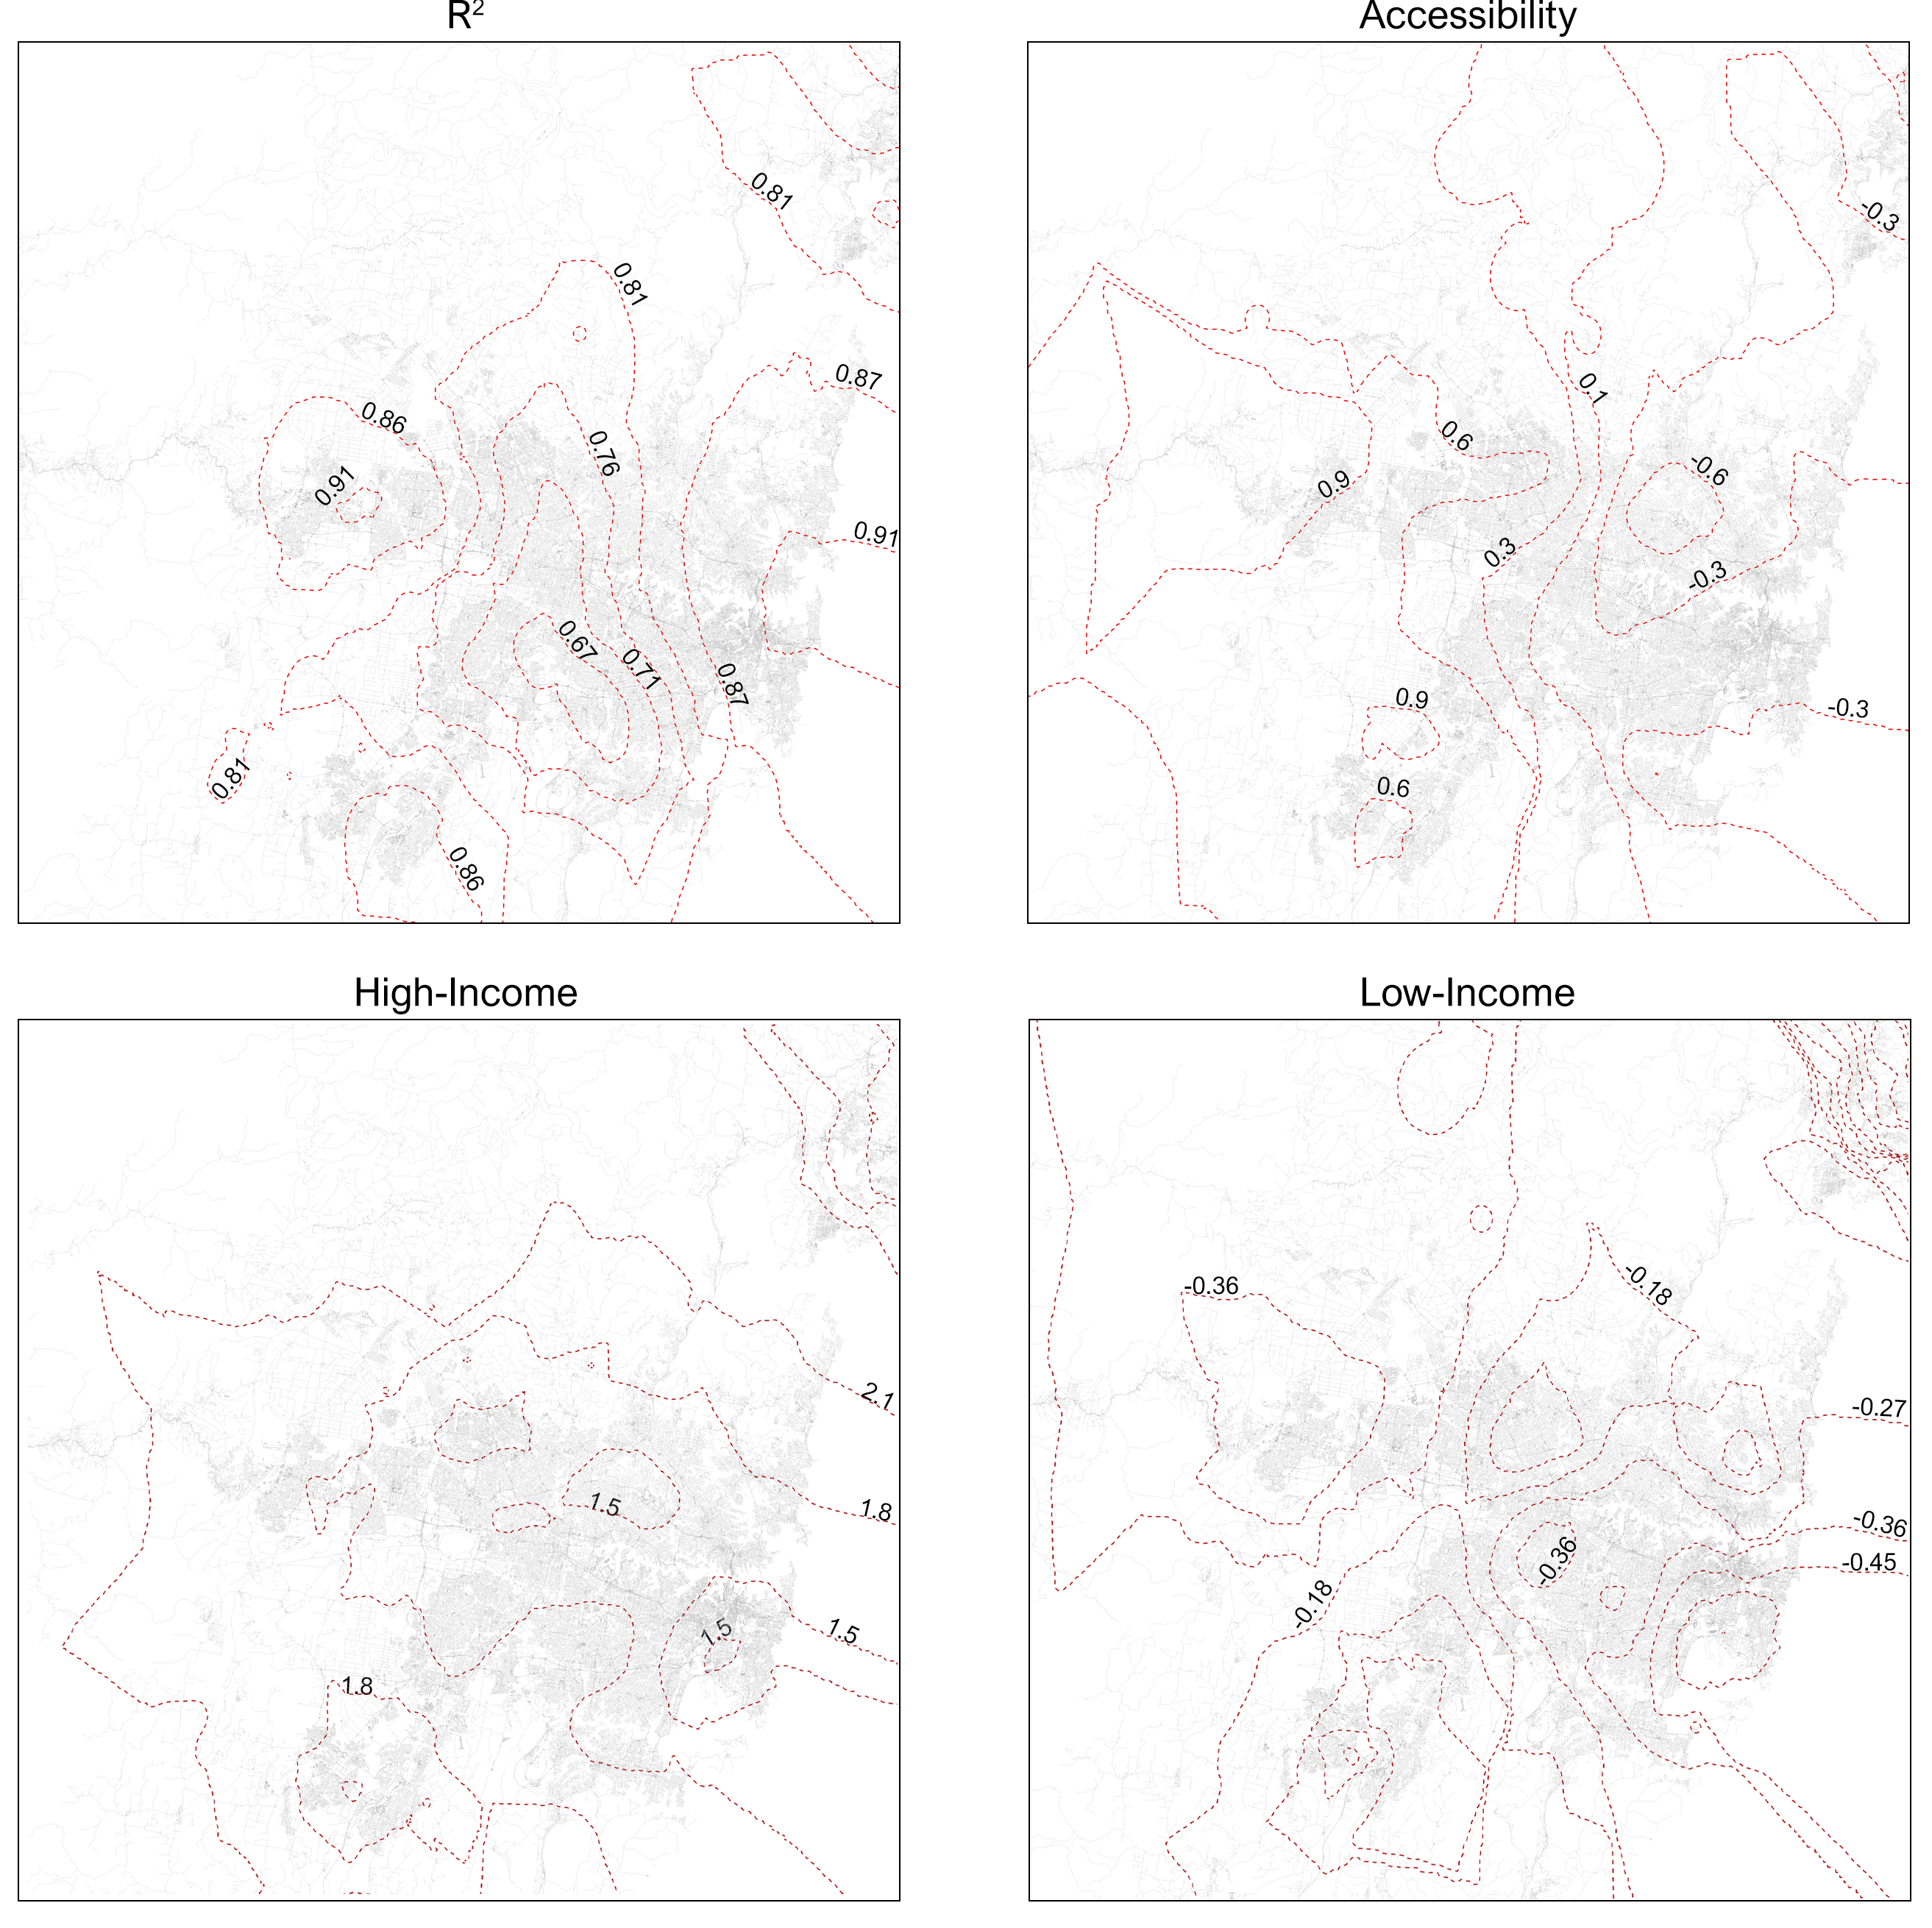
\includegraphics[width=1\textwidth]{body/figures/access_contour.png}
    \caption{Caption}
    \label{fig:gwr_accessibility_contour}
\end{figure}


Nevertheless, whilst the OLS model provides a relatively sound representation of house price variances at the metropolitan, their local effects also need to be considered with respect to the spatial non-stationarity of property. These local effects are considered within the subsequent GWR model. The GWR model specified here indicates an improvement in performance, with a adjusted $R^2$ value of 0.844 and a lowered residual sum of squares value of 1,569. The spatial distribution of the local $R^2$ values, along with the coefficient estimates for accessibility, high-- and low-- income groups, is illustrated in Figure \ref{fig:gwr_accessibility_contour}. The GWR model performance tends to remain high, with at least 67 per cent of house price variances accounted across all GS metropolitan geographies.

\renewcommand{\baselinestretch}{0.8}
\begin{table}[!ht]
  \centering \small
    \begin{tabular}{lccccc}
    \multicolumn{6}{l}{Summary of GWR coefficient estimates:} \\
          & \multicolumn{1}{c}{\textbf{Min}} & \multicolumn{1}{c}{\textbf{1Q}} & \multicolumn{1}{c}{\textbf{Median}} & \multicolumn{1}{c}{\textbf{3Q}} & \multicolumn{1}{c}{\textbf{Max}} \\
    \midrule
    Intercept & \multicolumn{1}{c}{6.2E+00} & \multicolumn{1}{c}{1.3E+01} & \multicolumn{1}{c}{1.4E+01} & \multicolumn{1}{c}{1.4E+01} & \multicolumn{1}{c}{1.8E+01} \\
    Bedrooms & \multicolumn{1}{c}{1.1E-01} & \multicolumn{1}{c}{1.2E-01} & \multicolumn{1}{c}{1.4E-01} & \multicolumn{1}{c}{1.6E-01} & \multicolumn{1}{c}{1.9E-01} \\
    Bathrooms & \multicolumn{1}{c}{2.8E-02} & \multicolumn{1}{c}{4.0E-02} & \multicolumn{1}{c}{5.1E-02} & \multicolumn{1}{c}{5.8E-02} & \multicolumn{1}{c}{8.1E-02} \\
    Distance to Sydney & \multicolumn{1}{c}{-3.4E-05} & \multicolumn{1}{c}{-3.0E-05} & \multicolumn{1}{c}{-2.3E-05} & \multicolumn{1}{c}{-1.5E-05} & \multicolumn{1}{c}{0.0E+00} \\
    Distance to Secondary City & \multicolumn{1}{c}{-1.6E-05} & \multicolumn{1}{c}{-4.7E-06} & \multicolumn{1}{c}{-5.6E-07} & \multicolumn{1}{c}{4.1E-06} & \multicolumn{1}{c}{0.0E+00} \\
    Distance to Beach & \multicolumn{1}{c}{-3.8E-05} & \multicolumn{1}{c}{-8.7E-06} & \multicolumn{1}{c}{2.3E-06} & \multicolumn{1}{c}{8.7E-06} & \multicolumn{1}{c}{0.0E+00} \\
    Distance to Bus Interchanges & \multicolumn{1}{c}{-3.8E-05} & \multicolumn{1}{c}{-9.7E-06} & \multicolumn{1}{c}{-3.2E-06} & \multicolumn{1}{c}{4.4E-06} & \multicolumn{1}{c}{0.0E+00} \\
    Distance to Highway & \multicolumn{1}{c}{-1.8E-05} & \multicolumn{1}{c}{3.0E-06} & \multicolumn{1}{c}{7.6E-06} & \multicolumn{1}{c}{1.1E-05} & \multicolumn{1}{c}{0.0E+00} \\
    Distance to Primary School & \multicolumn{1}{c}{-3.7E-05} & \multicolumn{1}{c}{1.3E-05} & \multicolumn{1}{c}{2.7E-05} & \multicolumn{1}{c}{4.5E-05} & \multicolumn{1}{c}{1.0E-04} \\
    Distance to University & \multicolumn{1}{c}{-2.1E-05} & \multicolumn{1}{c}{2.3E-06} & \multicolumn{1}{c}{6.5E-06} & \multicolumn{1}{c}{1.1E-05} & \multicolumn{1}{c}{0.0E+00} \\
    Distance to Swimming Pool & \multicolumn{1}{c}{-2.7E-05} & \multicolumn{1}{c}{-1.3E-05} & \multicolumn{1}{c}{-4.5E-06} & \multicolumn{1}{c}{6.8E-06} & \multicolumn{1}{c}{0.0E+00} \\
    Distance to Shopping Centres & \multicolumn{1}{c}{-1.5E-05} & \multicolumn{1}{c}{-4.0E-07} & \multicolumn{1}{c}{7.2E-06} & \multicolumn{1}{c}{1.8E-05} & \multicolumn{1}{c}{0.0E+00} \\
    Distance to Sports Centres & \multicolumn{1}{c}{-1.2E-05} & \multicolumn{1}{c}{3.6E-06} & \multicolumn{1}{c}{6.7E-06} & \multicolumn{1}{c}{1.4E-05} & \multicolumn{1}{c}{0.0E+00} \\
    Population Above 65 & \multicolumn{1}{c}{1.2E-03} & \multicolumn{1}{c}{2.6E-03} & \multicolumn{1}{c}{3.7E-03} & \multicolumn{1}{c}{5.8E-03} & \multicolumn{1}{c}{8.9E-03} \\
    Crime Rate & \multicolumn{1}{c}{-3.1E-01} & \multicolumn{1}{c}{-8.0E-02} & \multicolumn{1}{c}{-2.1E-02} & \multicolumn{1}{c}{1.0E-01} & \multicolumn{1}{c}{6.8E-01} \\
    Low Income (\%) & \multicolumn{1}{c}{-7.2E+00} & \multicolumn{1}{c}{-3.8E-01} & \multicolumn{1}{c}{-2.8E-01} & \multicolumn{1}{c}{-1.6E-01} & \multicolumn{1}{c}{5.0E+00} \\
    Middle Income (\%) & \multicolumn{1}{c}{-6.6E+00} & \multicolumn{1}{c}{-3.1E-01} & \multicolumn{1}{c}{-1.8E-01} & \multicolumn{1}{c}{-6.7E-02} & \multicolumn{1}{c}{5.4E+00} \\
    High Income (\%) & \multicolumn{1}{c}{-4.5E+00} & \multicolumn{1}{c}{1.5E+00} & \multicolumn{1}{c}{1.7E+00} & \multicolumn{1}{c}{1.8E+00} & \multicolumn{1}{c}{7.7E+00} \\
    Accessibility Score & \multicolumn{1}{c}{-7.8E-01} & \multicolumn{1}{c}{-2.8E-01} & \multicolumn{1}{c}{3.3E-04} & \multicolumn{1}{c}{5.7E-01} & \multicolumn{1}{c}{1.1E+00} \\
    \midrule
    Diagnostic information &       &       &       &       &  \\
    \multicolumn{6}{l}{\textit{Number of data points: 32,068 }} \\
    \multicolumn{6}{l}{\textit{Effective number of parameters: 192.2415 }} \\
    \multicolumn{6}{l}{\textit{Effective degrees of freedom: 31,875.76 }} \\
    \multicolumn{6}{l}{\textit{AICc: -5,447.286 }} \\
    \multicolumn{6}{l}{\textit{AIC: -5,594.308 }} \\
    \multicolumn{6}{l}{\textit{Residual sum of squares: 1,569.958 }} \\
    \multicolumn{6}{l}{\textit{R-square value:  0.8458043 }} \\
    \multicolumn{6}{l}{\textit{Adjusted R-square value:  0.8448744}} \\
    \end{tabular}%
    \caption{Add caption}
  \label{tab:GWR_coeffs}%
\end{table}

A summary of the model's coefficient estimates is also provided in Table \ref{tab:GWR_coeffs}. The findings here provide a more granular estimate of the model's income and accessibility effects --- in which, larger spatial disparities at local-levels are more evident than previously indicated in the OLS model. First, with respect to accessibility, the model's estimate coefficients  show a clear divide between the east and west regions of GS. In those areas to the West, the coefficient estimates actually indicate a negative relationship to house price. These findings suggest that accessibility may not necessarily be an important determinant of house prices, given its relatively equal distribution as aforementioned. Rather, where accessibility may perhaps be a more important factor are those locations more distal to Sydney's primary important centres. In these areas (e.g., Mount Druitt, Blacktown, Penrith), model estimates show up to a 0.9 per cent increase in house prices as accessibility improves. \\

What is also evident from the model estimates are the divide seen with income groups. The GWR results indicate a median decrease of 0.28 per cent associated within increasing proportions of low-income earners; whereas, a median increase of 1.7 per cent in noted with properties found in predominantly high-income areas. However, it is interesting to note the coefficient changes in areas like Sydney's Eastern suburbs. In these relative higher priced areas, the GWR indicates that any small increase in low-income groups within the area has an overwhelmingly detrimental effect on house prices than seen in the suburbs of Sydney's West-- and Inner-West--. In comparison to the coefficient estimates of computed for high-income groups, the findings suggest that house prices tend to be notably more sensitive to the presence of high-income groups. Model estimates in these areas indicate house price increases between 1.5 to 2.1 per cent, in comparison to the 0.18 to 0.45 per cent decreases seen with lower-income areas.

\section{Conclusion}
 
 